  %%%%%%%%%%%%%%%%%%%%%%%%%%%%%%%%%%%%%%%%%%%%%%%%%%%%%%%%%%%%%%%%
%                                                              %
%   ECCE Note template
%   v0 produced August 1, 2021
%             
%                                                              %
%%%%%%%%%%%%%%%%%%%%%%%%%%%%%%%%%%%%%%%%%%%%%%%%%%%%%%%%%%%%%%%%

%%  ECCE proposal team: Peter Steinberg (peter.steinberg@bnl.gov)

% C. Fanelli --- Oct 8, re-adapted template
 
                           
\documentclass[12pt,twoside]{article}
%\date{December 1, 2021}

%-----------
\usepackage{array}
\newcolumntype{P}[1]{>{\centering\arraybackslash}p{#1}}
\newcolumntype{M}[1]{>{\centering\arraybackslash}m{#1}}

%%%%%%%%%%%%%%%%
% Adding the include only list allows you to typeset only your
% chapter while maintaining overall page numbers and references.
% It also shields you from errors in other chapters as you go along.
% You need to typeset the whole thing once though. 

%\includeonly{title_page,daq_trig/daq_trig}

%%%%%%%%%%%%%%%%%%  header  (packages, 
%%%%%% Header for sPHENIX Conceptual Design Report -- 2017 

\RequirePackage{lineno}
\usepackage{import}
%\usepackage{titlesec}
\usepackage{enumitem}
\usepackage{amssymb, amsmath}
\usepackage{mathpazo}
\usepackage{float,graphicx}
%\graphicspath{{./}{pCDR/}}
\usepackage[figuresright]{rotating}
\usepackage{wrapfig}
\usepackage[usenames,dvipsnames]{color}
\usepackage{microtype}
\usepackage{tabulary}
%\usepackage{booktabs,multirow,dcolumn,bigdelim}
\newcommand{\otoprule}{\midrule[\heavyrulewidth]}
\usepackage{xr-hyper}
\usepackage[pdftex,plainpages=false,pdfpagelabels,backref,pdfborder={0 0 0}]{hyperref}
%\usepackage{hyperref}
\usepackage{url}
\usepackage[toc,page,titletoc]{appendix}
%\usepackage{afterpage}
\usepackage[font=small,labelfont=bf]{caption}
\setlength\captionmargin{15pt}
\usepackage[scaled]{helvet}
\usepackage{sectsty}
\allsectionsfont{\normalfont\sffamily}
%\usepackage{titletoc}
\usepackage{bytefield}
\usepackage{verbatimbox}
%\titlecontents{chapter}
%  [1.5em]
%  {\linespread{0.9}\normalfont\sffamily\bfseries}
%  {\contentslabel{1em}} 
%  {\hspace*{-1.3em}} 
%  {\mdseries\titlerule*[1pc]{.}\contentspage} 
%\titlecontents{section}
%  [3.5em]
%  {\linespread{0.9}\normalfont\sffamily}
%  {\contentslabel{2.3em}} 
%  {\hspace*{-2.3em}} 
%  {\titlerule*[1pc]{.}\contentspage} 
%\titlecontents{subsection}
%  [4.5em]
%  {\linespread{0.9}\normalfont\sffamily}
%  {\contentslabel{2.3em}} 
%  {\hspace*{-2.3em}} 
%  {\titlerule*[1pc]{.}\contentspage} 
%\titlecontents{subsubsection}
%  [5.5em]
%  {\linespread{0.9}\normalfont\sffamily}
%  {\contentslabel{2.3em}} 
%  {\hspace*{-2.3em}} 
%  {\titlerule*[1pc]{.}\contentspage} 
%\tolerance = 10000

\usepackage[text={6.5in,8.75in},headheight=26pt,centering]{geometry}
\usepackage{xspace}

\DeclareGraphicsExtensions{.pdf,.png}
\newcommand{\filenamedot}{.}
\setlength{\parindent}{0.0in}
\setlength{\parskip}{0.1in}
\renewcommand{\topfraction} {0.9}
\renewcommand{\bottomfraction} {0.9}
\renewcommand{\textfraction} {0.1}
\renewcommand{\floatpagefraction} {0.8}

%\usepackage{fancyhdr}
%\pagestyle{fancy}
%\renewcommand{\chaptermark}[1]{\markboth{#1}{}}
%\renewcommand{\sectionmark}[1]{\markright{#1}{}}
%\fancyhead{} % clear all header fields 
%\fancyhead[RO,LE]{\sffamily \rightmark}
%\fancyhead[LO,RE]{\sffamily \leftmark}
%\fancyfoot{} % clear all footer fields 
%\fancyfoot[RO,LE]{\sffamily \thepage}
%\renewcommand{\headrulewidth}{0pt} 
%\fancypagestyle{plain}{%
%  \fancyhf{}
%  \fancyfoot[RO,LE]{\sffamily \thepage}
%}

\usepackage{multirow}
\usepackage{eurosym}
\usepackage{xcolor}
\usepackage{framed}
\colorlet{shadecolor}{blue!10}

\usepackage{gensymb}

\setcounter{secnumdepth}{3}
\setcounter{tocdepth}{1}

\newcommand{\martinimusic}{\mbox{\sc Martini+Music}\xspace}
\newcommand{\hic}{\mbox{$A$$+$$A$}\xspace}
\newcommand{\pA}{\mbox{$p$$+$$A$}\xspace}
\newcommand{\AuAu}{\mbox{Au$+$Au}\xspace}
\newcommand{\auau}{\mbox{Au$+$Au}\xspace} 
\newcommand{\raa}{\mbox{$R_\mathrm{AA}$}\xspace}
\newcommand{\pbpb}{\mbox{Pb$+$Pb}\xspace} 
\newcommand{\pdau}{\mbox{$p(d)$$+$Au}\xspace} 
\newcommand{\pau}{\mbox{$p$$+$Au}\xspace} 
\newcommand{\aj}{\mbox{$A_J$}\xspace} 
\newcommand {\pp}{\mbox{$p$$+$$p$}\xspace}
\newcommand {\ppbar}{\mbox{$p$$+$$\overline{p}$}\xspace}
\newcommand{\pT}{\mbox{${p_T}$}\xspace}
\newcommand{\jpsi}{\mbox{$J/\psi$}}
\newcommand{\sqrtsnn}{\mbox{$\sqrt{s_{\scriptscriptstyle NN}}$}}
\newcommand{\npart}{$N_\mathrm{part}$}
\newcommand{\ncoll}{$N_\mathrm{coll}$}
\newcommand{\qgp}{\mbox{quark-gluon plasma}\xspace}
\newcommand{\jt}{\mbox{$J_T$}} \newcommand{\qhat}{\mbox{$\hat{q}$}}
\newcommand{\Qsqr}{\mbox{$Q^2$}} \newcommand{\CuCu}{\mbox{Cu$+$Cu}}
\newcommand{\PbPb}{\mbox{Pb$+$Pb}} \newcommand{\pPb}{\mbox{$p$$+$Pb}}
\newcommand{\gjet}{\mbox{$\gamma$-jet}}
\newcommand{\Qmax}{\mbox{$Q_{\max}$}} \newcommand{\ET}{\mbox{$E_T$}}
\newcommand{\Et}{\mbox{$E_T$}} \newcommand{\kt}{\mbox{$k_T$}}
\newcommand{\RAA}{\mbox{$R_{AA}$}\xspace} \newcommand{\IAA}{\mbox{$I_{AA}$}}
\newcommand{\pt}{\mbox{${p_T}$}\xspace}
\newcommand{\highpt}{high-${\rm p_{_{T}}}$}
\newcommand{\lessim}{{\stackrel{<}{\sim}}} \newcommand{\eqnpt}{p_T}
\newcommand{\eA}{\mbox{$e-{\rm A}$}}
\newcommand{\dAu}{\mbox{$d$$+$Au}\xspace}
\newcommand{\pAu}{\mbox{$p$$+$Au}\xspace}
\newcommand{\GeVSQ}{\mbox{${\rm GeV}^2$}}
\newcommand{\fastjet}{\mbox{\sc FastJet}\xspace}
\newcommand{\geant}{\mbox{\sc Geant4}\xspace}
\newcommand{\antikt}{\mbox{anti-$k_T$}\xspace}
\newcommand{\pythia}{\mbox{\sc Pythia}\xspace}
\newcommand{\opera}{\mbox{\sc Opera}\xspace}
\newcommand{\rapgap}{\mbox{\sc Rapgap}\xspace}
\newcommand{\milou}{\mbox{\sc Milou}\xspace}
\newcommand{\pyquen}{\mbox{\sc Pyquen}\xspace}
\newcommand{\hijing}{\mbox{\sc Hijing}\xspace}
\newcommand{\roofit}{\mbox{\sc RooFit}\xspace}
\newcommand{\roounfold}{\mbox{\sc RooUnfold}\xspace}
\newcommand{\beetle}{\mbox{\sc Beetle}\xspace}
\newcommand{\gj}{\mbox{$\gamma$+jet}\xspace}
\newcommand{\gh}{\mbox{$\gamma$+hadron}\xspace}
\newcommand{\martini}{\mbox{\sc Martini}\xspace}
\newcommand{\music}{\mbox{\sc Music}\xspace}
\newcommand{\Ephenix}{Electron-Ion Collider (EIC) detector built
 around the BaBar magnet and sPHENIX calorimetry\xspace}
\newcommand{\ephenix}{EIC detector built around the BaBar magnet and
 sPHENIX calorimetry\xspace} 
\newcommand{\refdesign}{reference design\xspace}
\newcommand{\refconfig}{reference configuration\xspace}
\newcommand{\dijet}{\mbox{dijet}\xspace}
\newcommand{\fake}{\mbox{fake}\xspace}
\newcommand{\fast}{\mbox{fast}\xspace}
\newcommand{\veryfast}{\mbox{very fast}\xspace}
\newcommand{\epem}{\mbox{$e^+e^-$}\xspace}
\newcommand{\onewidth}{0.6\linewidth}
\newcommand{\twowidth}{0.48\linewidth}
\newcommand{\threewidth}{0.32\linewidth}
\newcommand{\egoing}{\mbox{electron-going}\xspace}
\newcommand{\hgoing}{\mbox{hadron-going}\xspace}
\newcommand{\egodir}{electron-going direction\xspace}
\newcommand{\hgodir}{hadron-going direction\xspace}

\newcommand{\red}{\color{red}}
\newcommand{\blue}{\color{blue}}	 
\newcommand{\green}{\color{green}}	 
\newcommand{\magenta}{\color{magenta}}

\newcommand{\lyxdot}{.}
\usepackage{subfig}

\setlength\fboxsep{0pt}
\setlength\fboxrule{0.5pt}

\usepackage[textwidth=1in,textsize=footnotesize,disable]{todonotes}
%\usepackage[textwidth=1in,textsize=footnotesize]{todonotes}


\title{ECCE Computing Plan}
\author[1,2,3]{Jan C. Bernauer}
\author[4]{Cameron Dean}
\author[5]{Cristiano Fanelli}
\author[6]{Jin Huang}
\author[6]{Kolja Kauder}
\author[7]{David Lawrence}
\author[6,8]{Joseph D. Osborn}
\author[5]{Christoph Paus}

 \renewcommand\Affilfont{\itshape\small}
\affil[1]{Department of Physics and Astronomy, Stony Brook University, Stony Brook, NY, USA}
\affil[2]{RIKEN BNL Research Center, Upton, NY, USA}
\affil[3]{Center for Frontiers in Nuclear Science, Stony Brook University, Stony Brook, NY, USA}
\affil[4]{Los Alamos National Laboratory, Los Alamos, NM, USA}
\affil[5]{Laboratory for Nuclear Science, Massachusetts Institute of Technology, Cambridge, MA, USA}
\affil[6]{Brookhaven National Laboratory, Upton, NY, USA}
\affil[7]{Thomas Jefferson National Accelerator Facility, Newport News, VA, USA}
\affil[8]{Oak Ridge National Laboratory, Oak Ridge, TN, USA}




\begin{document}
%\frontmatter
%\pagestyle{empty} %Setting this to empty removes page numbers
\pagestyle{empty}
%%%%%%%%%%%%%%%%%%%%%%%%%%%%%%%%% title page
\renewcommand*\familydefault{\sfdefault}
{\sffamily
\vfill
\vspace{4cm}
\begin{figure}[H]
  \begin{center}
  
\includegraphics[width=0.3\linewidth]{figs/ecce-logo.png}
\end{center}
\end{figure}

\begin{center}
  \large
  {\LARGE{ECCE Computing Plan}}

  \begin{tabular}{cc}

%A full-acceptance detector at the EIC based on the BaBAR magnet 
& \today%December 1, 2021 \\
  \end{tabular}
  \end{center}

\vspace{15cm}
\hspace*{0pt}\hfill ecce-note-comp-2021-01 \\
\hspace*{0pt}\hfill v1.0
\vspace{-15cm}

\vspace{1cm}

\begin{figure}[H]
  \begin{center}
    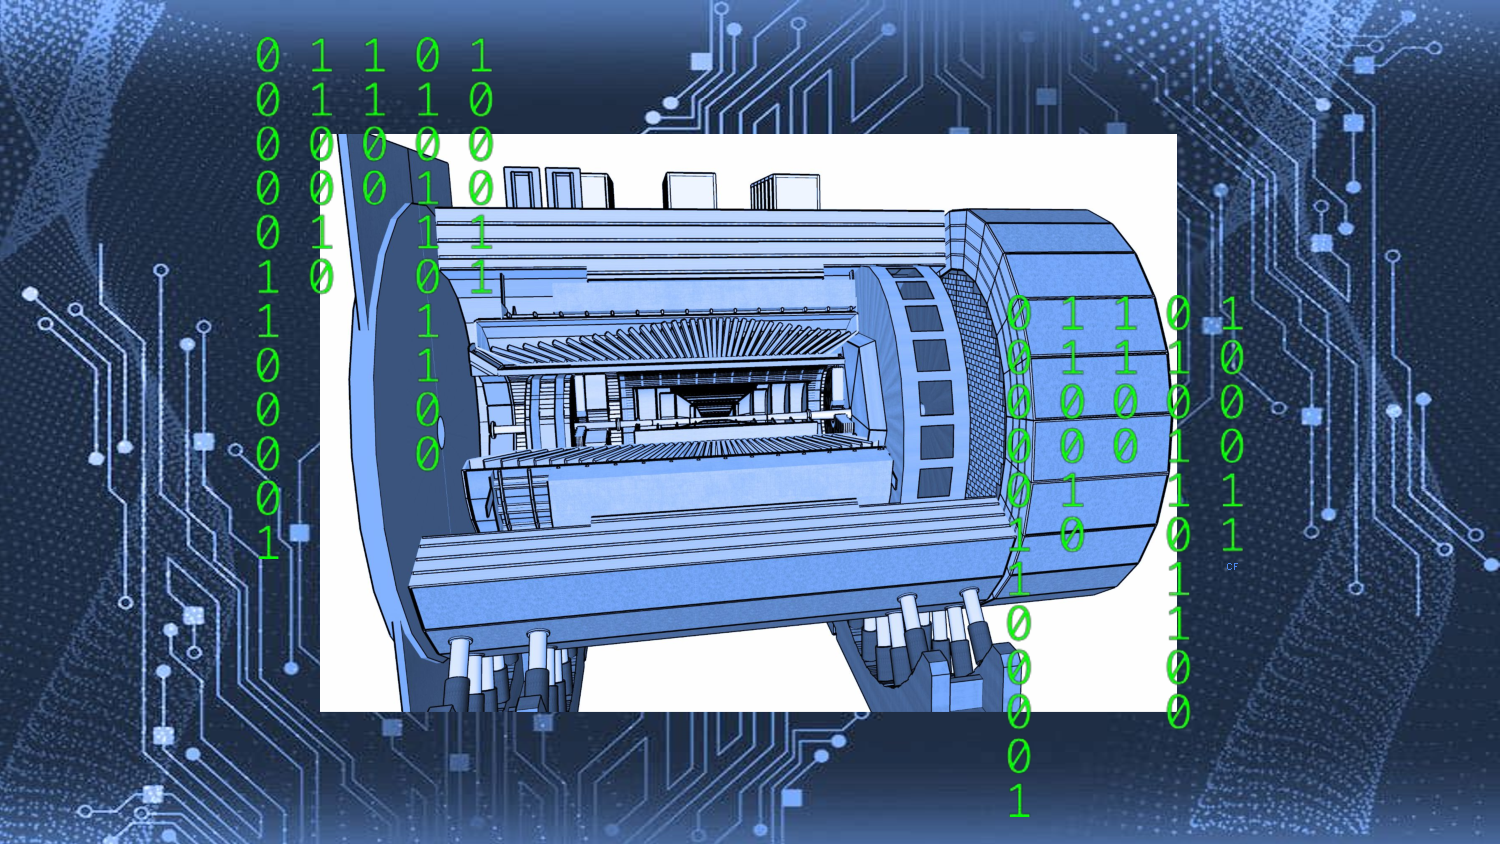
\includegraphics[width=0.9\linewidth]{figs/ECCE_Computing_Fig2.pdf}
  \end{center}
\end{figure}
}


\vfill
\renewcommand*\familydefault{\rmdefault}


\cleardoublepage
\pagestyle{plain}
\maketitle
\pagenumbering{roman}

%\setcounter{page}{1}

%\clearpage
%\cleardoublepage

%\resetlinenumber


%\cleardoublepage

%\mainmatter

%\renewcommand{\thepage}{\arabic{page}}
%\setcounter{chapter}{0}
%\setcounter{page}{1}

%%%%%%%%%%%%%%%%%%%%%%%%%%%%%%%%% 
\begin{abstract}
%\section* {Executive Summary}
\label{sec:ExecutiveSummary}

% Executive Summary

The ECCE consortium plans to deploy a federated computing model for the EIC where multiple facilities are used. ECCE recognizes the need for a global EIC model and intends to fully participate in the design and implementation of such a system. A similar strategy has been successfully deployed by the LHC in the form of the Worldwide LHC Computing Grid (WLCG)~\cite{SHIERS2007219}. ECCE has developed a tiered ``Butterfly'' model for EIC computing that was inspired by the WLCG model, but updated to better reflect the computing landscape anticipated for the EIC. In this model, the EIC detector supplies the data, but the SDCC at BNL is treated as one of a pool of sites used for long term storage and compute. Both SDCC and JLab would be considered as \emph{Echelon 1} sites with the ability to add others as appropriate. Raw data would be distributed amongst multiple \emph{Echelon 2} sites for processing with the processed data being returned to Echelon 1. Researchers would directly access the processed data at the Echelon 1 sites.

We have adopted a fixed-latency offline computing model where both the final calibration and reconstruction of raw data occur within 2-3 weeks of acquisition. During this period, raw data will be buffered on disk at all of the Echelon 1 sites, along with permanent archival copies on tapes. Final calibration will be performed semi-automatically including accumulating sufficient data for tracker alignment and energy scale calibration of the calorimeters. AI/ML will be integrated throughout this model. After calibration, data processing  will be released to multiple sites including HTC facilities at both Echelon 1 and 2 sites. We expect that the produced simulation sample will focus on 10\% of the EIC collision cross-section that is directly relevant for the signal and background of the core ECCE physics program. These physics processes will be simulated to $O(10)$~times the statistics in real data to constrain systematic uncertainty from the simulated sample to be much smaller than the data statistical uncertainty.

A summary of the anticipated resource requirements can be seen here in table \ref{tab:computing-integrated_luminosity_by_year}.


\begin{table}[htb!]
    %\centering
    \hskip-0.8cm
    \begin{tabular}{c|c|c|c}
        \hline
        % \hline
         \textbf{ECCE Runs}       & year-1                & year-2                  & year-3                \\
        \hline
         Luminosity              & $10^{33}\mathrm{cm}^{-2}\mathrm{s}^{-1}$ & $2\times 10^{33}\mathrm{cm}^{-2}\mathrm{s}^{-1}$ & $10^{34}\mathrm{cm}^{-2}\mathrm{s}^{-1}$ \\
        %  \hline
         Weeks of Running        & 10                    & 20                      & 30                    \\
        %  \hline
         Operational efficiency    & 40\%                  & 50\%                    & 60\%                  \\
        %  \hline
        Disk (temporary)  &  1.2PB & 3.0PB & 18.1PB \\
        %\hline
        Disk (permanent)    & 0.4PB & 2.4PB &	20.6PB \\
        %\hline
        %\textbf{TOTAL}          & 1.6PB &	5.4PB &	38.7PB \\
         Data Rate to Storage    & 6.7Gbps               & 16.7Gbps                & 100Gbps               \\
        %  \hline
         Raw Data Storage (no duplicates) & 4PB          & 20PB                    & 181PB                 \\
        %  \hline
        %  Total Storage (no duplicates) & 4.4PB           & 22PB                   & 200PB                  \\
        %  \hline
        \hline
        Recon process time/core	& 5.4s/ev	& 5.4s/ev	& 5.4s/ev \\
        % \hline
        Streaming-unpacked event size	& 33kB	& 33kB & 33kB \\
        % \hline
        Number of events produced &	121 billion	& 605 billion & 5,443 billion \\
        % \hline
         Recon Storage          & 0.4PB                  & 2PB                    & 18PB                   \\
        %  \hline
        % CPU-core hours (recon-only, 1 pass)	& 24Mcore-hrs	& 121Mcore-hrs &	1089Mcore-hrs \\
        % \hline
        % CPU-core hours (calib-only) &	1.2Mcore-hrs &	6.0Mcore-hrs &	54.4Mcore-hrs \\	
        % \hline
        CPU-core hours (recon+calib)	& 191Mcore-hrs	& 953Mcore-hrs &	8,573Mcore-hrs \\
        % \hline
        2020-cores needed to process in 30 weeks	& 38k &	189k &	1,701k \\
        % \hline
        \hline
   \end{tabular}
    \caption{Estimate of raw data storage and compute needs for first 3 years of ECCE,  assuming ramp up to full luminosity by year 3. 
    % Numbers for the first two years are estimated for the purposes of this exercise and do not come from an external source. n.b. each value represents \emph{only} the needs for data produced in that year and \emph{not} a cumulative total.
    }
    \label{tab:computing-integrated_luminosity_by_year}
\end{table}

\end{abstract}
\clearpage
\setcounter{tocdepth}{3}
\tableofcontents
\clearpage
\pagenumbering{arabic}
\setcounter{page}{1}

\section {Introduction}
\label{sec:introduction}

%\textbf{\emph{David L.}}

The Electron Ion Collider (EIC) is the next generation precision nuclear physics accelerator complex that is being constructed in the United States. The EIC is expected to start producing data in the early 2030's, and is unique as it will collide high energy polarized electrons with polarized protons and a wide range of nuclei. As such, it will introduce new paradigms in large scale nuclear physics experiments. Expected luminosities at the EIC will reach upwards of $10^{34}$ cm$^{-2}$s$^{-1}$; consequently, there will be an extremely large data sample to process. Recent efforts from modern collider physics experiments have shown the benefits of near real-time analysis~\cite{Benson_2015,Aaij_2019}. Therefore, there is a strong desire to develop software and computing infrastructure that reliably and quickly processes data for analysis. 



As the EIC will start taking data in nearly a decade, there are a number of new paradigms that have the opportunity to be explored in this software R\&D phase. An example of such a new paradigm is the use of Artificial Intelligence (AI) and machine learning (ML). The EIC has the unique opportunity to be one of the first large-scale facilities to systematically incorporate and employ AI, starting from the detector design and R\&D phases. The relevance of AI for the EIC has been highlighted among the \textit{Opportunities for Computing} of the EIC Yellow Report \cite{YellowReport}. AI potentially permeates all aspects of this Computing Plan; in fact, it already plays a significant role in the design and R\&D phases of the EIC~\cite{cisbani2020ai}~\cite{AI4EIC2021}.

This document presents a proposed computing plan for the EIC Comprehensive Chromodynamics Experiment (ECCE) detector at the Electron-Ion Collider (EIC)~\cite{YellowReport}. This includes estimates of the rates from the detector, the pipeline for processing and storing the data, and how the collaboration members will access the data. Software systems for monitoring, calibration, reconstruction, and analysis are discussed. Estimates of the computing and storage requirements are included. AI detector optimization techniques are also discussed as this is expected to be a large part of the computing effort over the next few years. While we attempt to include some forward thinking plans in this regard, we necessarily do need to rely on past experience with other large experiments such as sPHENIX~\cite{sphenix_computing_plan_2019} and LHCb~\cite{CAMPORAPEREZ2016280} to serve as guides.








% temporarily commented --- CF
%\section {Artificial Intelligence / Machine Learning} %/Machine Learning
%\label{sec:ai}
%\textbf{\emph{Cristiano/Will}}
%
%\emph{This is intended to be a fairly brief section.
%AI/ML is expected to be integrated into all aspects of the Computing Plan so should appear throughout the document.
% }
%
%
%EIC 
%%has the possibility to incorporate AI from the start and 
%could be one of the first large-scale experiments where AI is systematically employed from the detector and design 

An example of such a new paradigm is the use of Artificial Intelligence (AI) and machine learning (ML) in its program. The EIC has the unique opportunity to be one of the first large-scale experiments to systematically incorporate and employ AI, starting from the detector design and R\&D phases. 
The relevance of AI for the EIC has been highlighted among the \textit{Opportunities for Computing} of the EIC Yellow Report \cite{eic_yellow_report_v1_1}. AI potentially permeates all aspects of the Computing Plan, and appears throughout this document; in fact, it already plays a significant role in the design and R\&D phases of the EIC~\cite{cisbani2020ai}.

%The first workshop on Artificial Intelligence for the Electron Ion Collider (AI4EIC) held at CFNS in September 2021 \cite{AI4EIC_workshop} has been a fundamental venue for the EIC community to start addressing how AI might contribute to advance research, design and operation of the future EIC across all the phases of the EIC schedule (see \cite{AI4EIC_future}).
%---- structure of AI4EIC 
%The workshop was structured into different sessions focusing on experimental applications of AI for \textit{Accelerator and Detector Design}, \textit{Simulations}, \textit{Reconstruction and Analysis}, \textit{Accelerator and Detector Control}, \textit{Detector Readout} and \textit{Computing Frontiers}. 



It is in fact clear the advantage of AI techniques in searching the optimal solutions in a complex multi-dimensional parameter space such as in the design of a detector. Detector design requires accurate simulations based on Geant4 \cite{ALLISON2016186}. Those simulations are typically compute intensive and another advantage of using AI is minimizing the computing budget needed to come up with an optimal solution (see, \textit{e.g.}, the results of an AI-supported design of a complex detector system like the dual-RICH \cite{cisbani2020ai}).
%AI can be also utilized for the optimization of materials used within detectors for improved performance. 

%Simulations - fast simulations - ATLAS example 

%The AI4EIC session on Simulations highlighted the need for faster simulations. The ATLAS Collaboration at CERN for example is already including a GAN \cite{creswell2018generative} in AtlFast3, the next generation of high-accuracy fast simulation in ATLAS \cite{atlas2021atlfast3}. 
%for fast simulations at intermediate energies.   
The EIC detector has unique features. For example, the backbone of particle identification is with imaging Cherenkov detectors \cite{he2020rich} (DIRC in the central region, mRICH in the e-going direction and dRICH in the h-going direction of the ECCE detector), which are typically characterized by compute intensive simulations and complex pattern recognition problems, that can benefit from novel AI-based approaches that have been recently proposed (see, \textit{e.g.}, \cite{fanelli2020deeprich}). %(see, \textit{e.g.}, \cite{ali2020gluex}).   
%
%
%
%Reconstruction - EIC detector has unique features. The backbone of PID is Cherenkov detectors. Compute intensive simulations and complex pattern recognition problems for imaging Cherenkov detectors like DIRC.  
 AI is also expected to play a role in high-level physics analysis, for example in jet physics to empower taggers for boosted jets and identify quark flavor within the jets (see ML4Jets workshops \cite{ml4jets}).    

%Another important aspect came from the Accelerator and Detector Control session of AI4EIC: in fact EIC can been envisaged as one the first experiments to be largely automated and endowed with intelligence in control workflows (see, \textit{e.g.}, \cite{Hydra2021} as discussed in Sec.~\ref{subsec:online_mon}).  

The EIC community is also moving towards a trigger-less Streaming Readout (SRO) approach to detector readout as discussed in Sec.~\ref{sec:online}. 
This represents a unique opportunity to streamline workflows for online and offline data processing in HEP and NP experiments, and to take advantage of emerging technologies such as \textit{e.g.}, heterogeneous computing with AI/ML as discussed in the Computing Frontiers session of AI4EIC.
Within the new paradigm of SRO, AI is expected to play a major role in providing fast alignment/calibration/reconstruction for near real-time analyses.

% What opportunities from “computing frontiers” in > 2030? 


%--- references to next sections go here ---

%--- few sentences to uncomment --- 

%--- Will: any addition?

%---- some numbers from:
%%CPU Resources
%%ECCE Tracker Optimization (Cristiano/Karthik)
%%DIRC Optimization Framework # of compute hours/configuration (Will/Andru)
%%Dual Rich (what used for the study in paper) (Cristiano)
%%General purpose simulation for generating training samples for projects listed below
%%???
%%GPU Resources
%%CLAS12 Tracking  (Gagik/ODU Students)
%%Hydra Online Monitoring Training (Kishan/Thomas)
%%Online track reconstruction?
%%???

%---- final summaries, keywords and citations 




% temporarily commented --- CF
%\section {Detector and Program Development}
%\label{sec:detector_development}
%\subsection{Detector Optimization}
\label{sec:codesign}
\textbf{\emph{Cristiano}}


Detector optimization is an essential part of the R\&D and design process that involves mechanical design and budget to realize the best performance possible.  
This process is anticipated to continue in the months following the detector proposal towards CD-2 and CD-3. 

Optimizing the design of large scale detectors like ECCE made by multiple sub-detector systems is a complex problem. 
Each sub-detector system is in fact characterized by a multi-dimensional design parameter space (describing, \textit{e.g.}, geometry, mechanics, optics, etc). 
In addition to that, detector simulations are typically computationally intensive, as we need to rely on advanced simulation platforms used in our community like Geant \cite{Agostinelli:2002hh} to simulate the interaction of radiation with matter. 

In the past the typical workflow during the design phase consisted in characterizing each sub-detector individually by taking into account constraints from the whole global detector design.
The optimization was usually carried out manually or with brute-force methods considering only one figure of merit. Eventually all sub-detectors were combined together.
Nowadays state of the art techniques based on AI can provide dedicated strategies for complex combinatorial searches. 
These algorithms are particularly useful to efficiently explore a usually large solution space and to minimize the computational budget needed to converge to these optimal solutions. 

The typical software stack that is utilized in the detector design process involves three main steps:
(i) generation of events, (ii) detector simulations
and (iii) reconstruction and analysis. 
%
A sequential AI-based strategy in general gathers the information associated to the proposed design point, \textit{i.e.} some figures of merit that quantify the goodness of the design, and based on this information suggests which design parameters to query at the next iteration. This scheme is shown in Fig.~\ref{fig:design_AI}. 
%
A first parallelized, automated and self-consistent AI-supported strategy for detector optimization has been demonstrated for the dual-RICH by \cite{cisbani2020ai} leveraging Bayesian optimization (BO) \cite{snoek2012practical}. 
A workflow of this framework is shown in Fig.~\ref{fig:dRICH_BO_scheme}, where more details can be found. 



\begin{figure}[!]
    \centering
    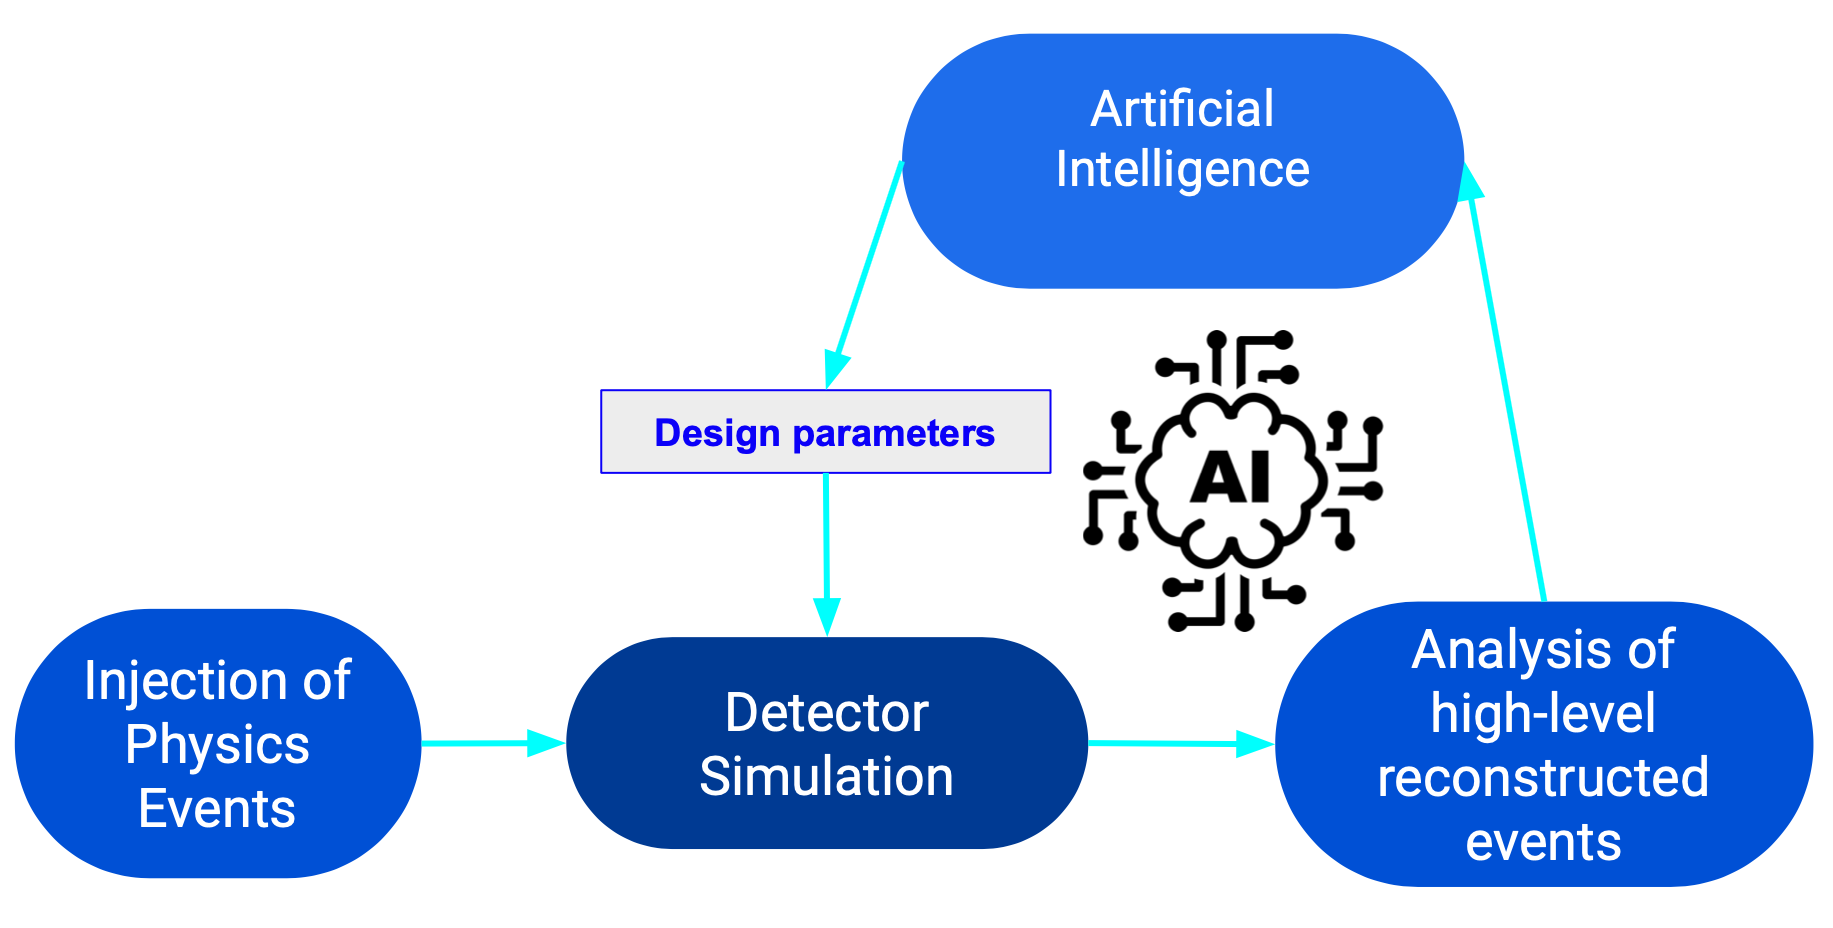
\includegraphics[scale = 0.18]{figs/design_workflow.png}
    %\includegraphics[scale = 0.15]{figs/ECCE_teams.png}
    \caption{%(top) 
    Typical workflow of detector design assisted by AI: physics events are injected in a detector characterized by some given design parameters. Reconstructed events are analyzed and figures of merit are quantified and passed to some AI-based strategy, which in turn suggests the next design point to observe in this sequential approach; notice that AI can also intervene in the simulation and reconstruction steps. %(bottom) AI fosters the interplay between the Detector, Physics and Computing Teams in ECCE: the Physics Team provides physics generators and is responsible for the evaluation of performance after reconstruction; the Detector Team is responsible of the selection of technology, the choice of the updated baseline design, and the proposal of alternative configurations; the Computing Team offers the support in producing the simulation campaign, as well as the optimization pipeline of each new alternative detector configuration.
    }
    \label{fig:design_AI}
\end{figure}

\begin{figure}[!]
    \centering
    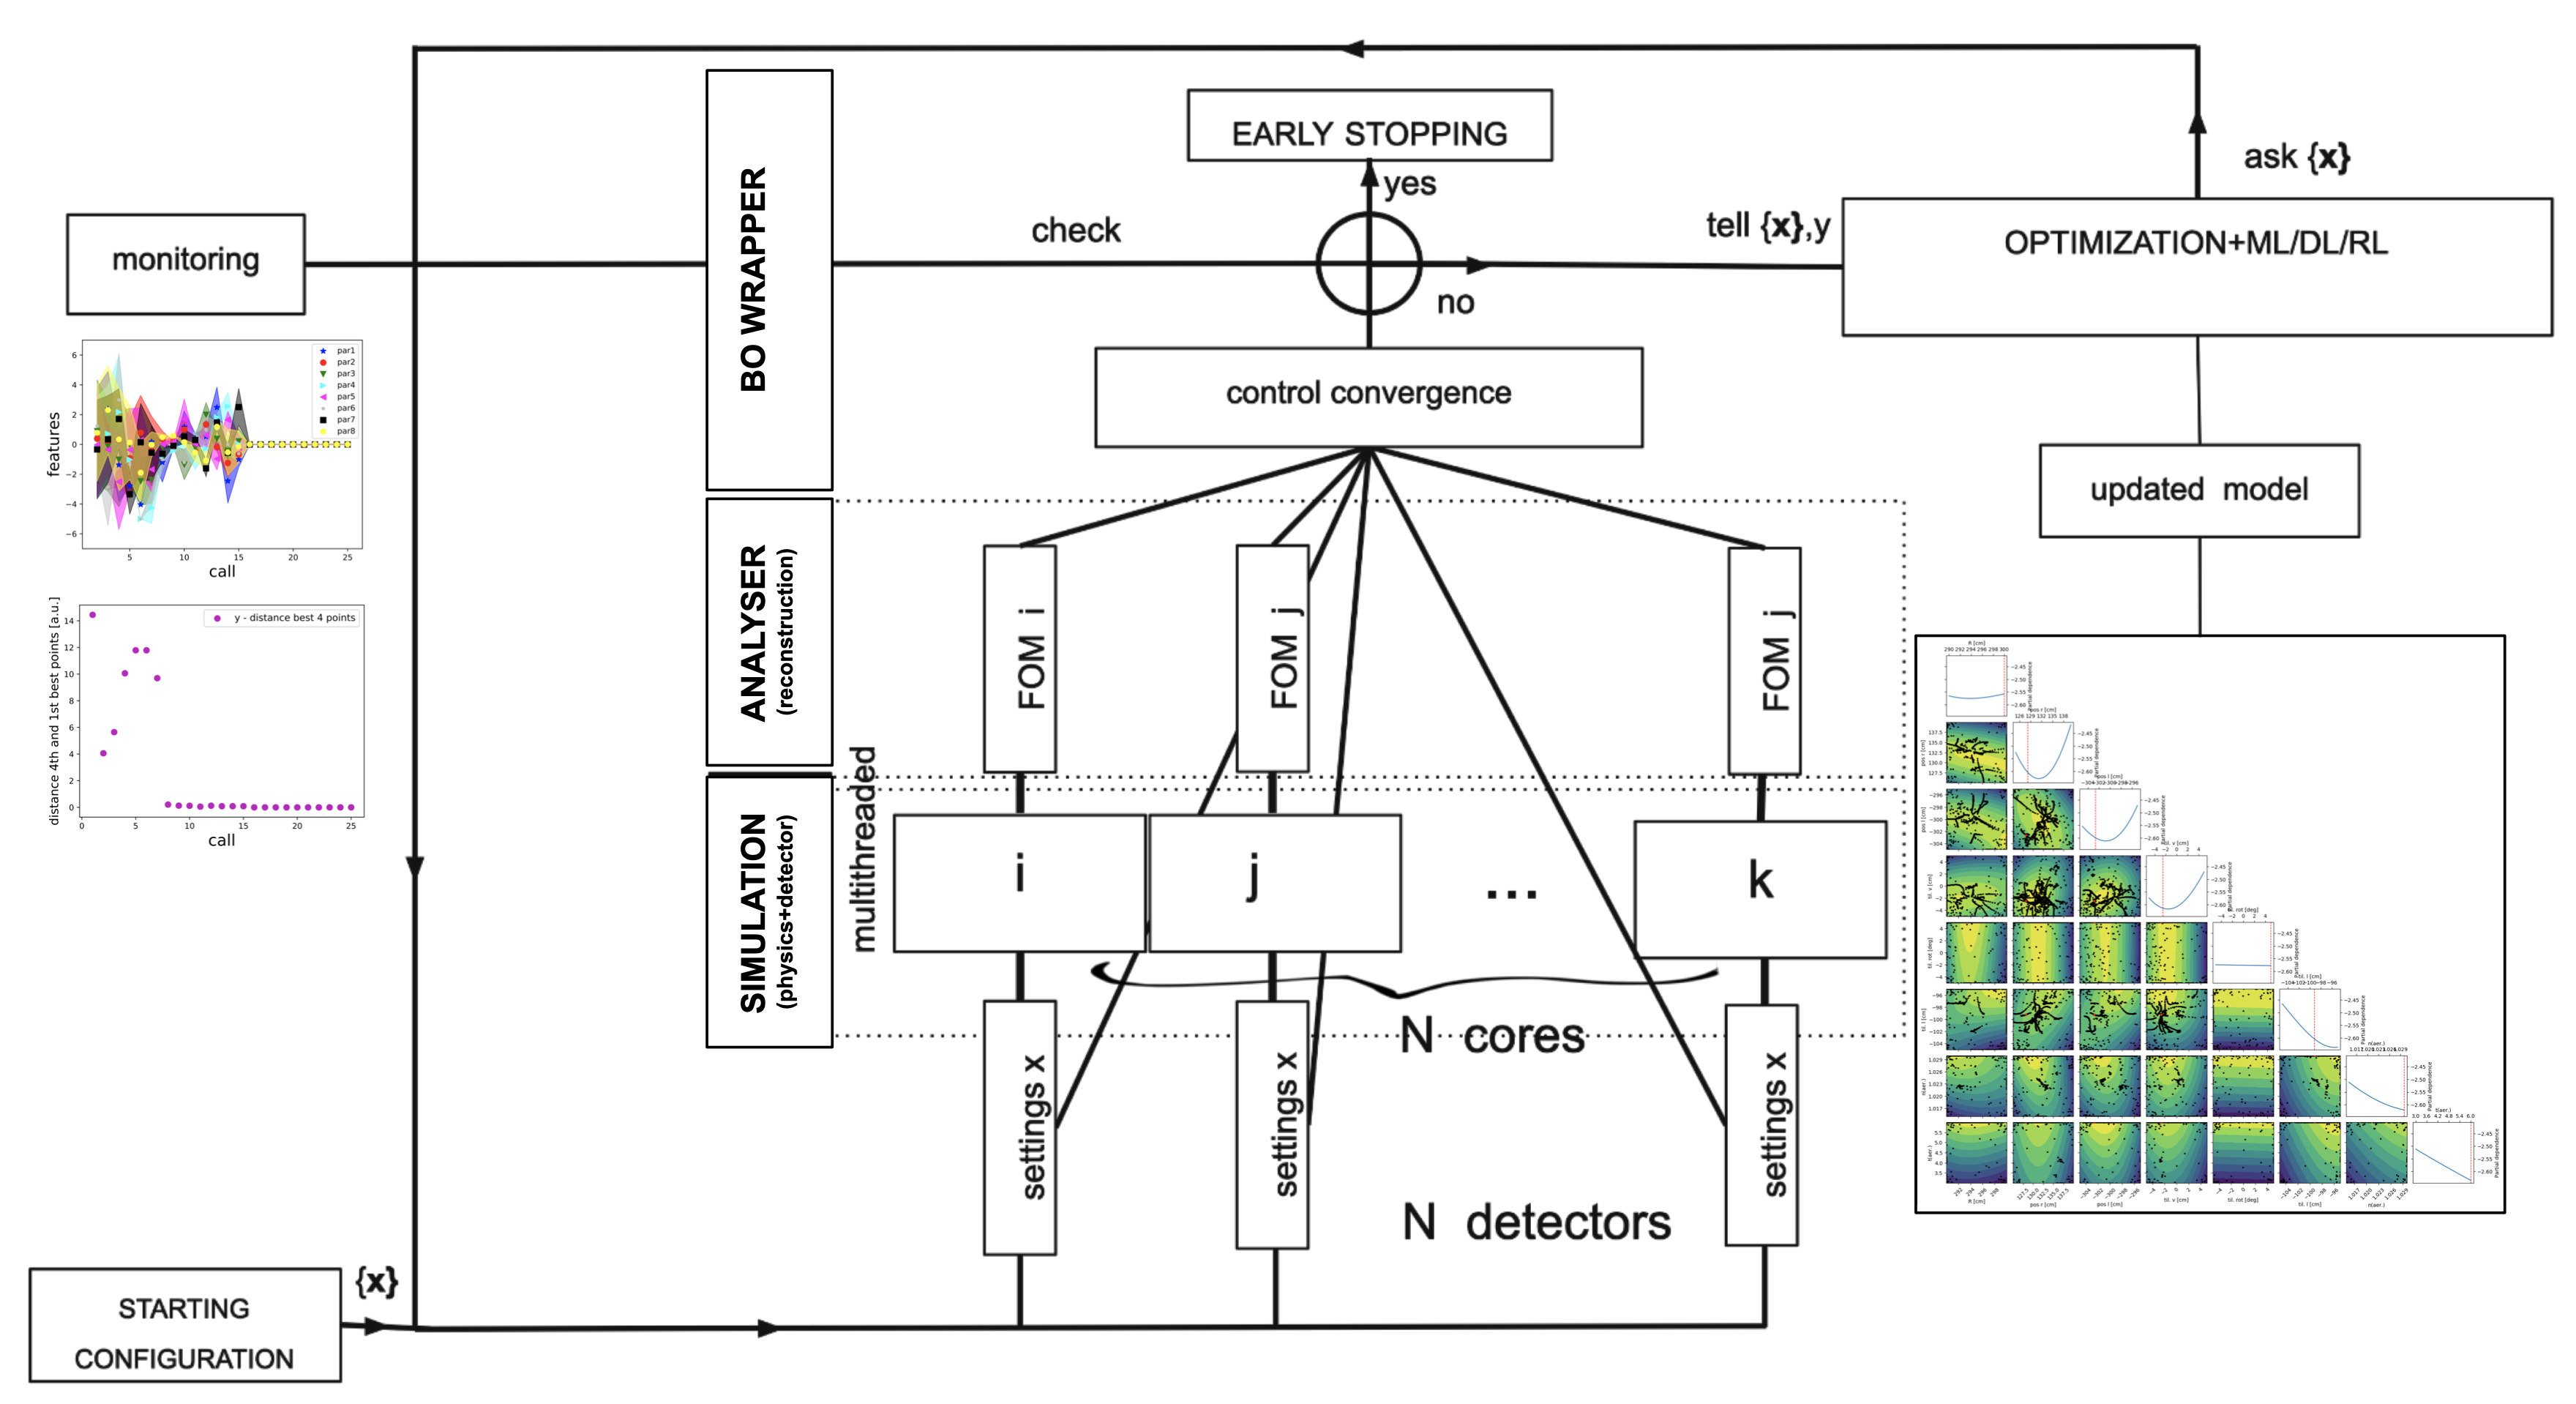
\includegraphics[scale = 0.21]{figs/dRICH_BO_scheme.png}
    \caption{
    Bayesian optimization framework for the optimization of the dual-RICH. N detector design points are created in parallel and passed to the BO which uses Gaussian processes, which collects the points, updates the surrogate model (a 2D visualization is shown in the bottom right corner considering all pairs of design parameters). A cheap acquisition function suggests new set of design points to query at the next iteration. Convergence criteria are implemented on both the design space and on the objective (in this case, the $\pi$/K separation power of the dual-RICH) and early stopping is activated when convergence is observed in both spaces. Figure taken from \cite{fanelli_jluo2021}. More details can be found in \cite{cisbani2020ai}.   
    }
    \label{fig:dRICH_BO_scheme}
\end{figure}

An unprecedented study in detector design using AI has been accomplished during the detector proposal and a framework for multi-objective optimization of the ECCE design has been developed. 
Our approach deals with a complex optimization in a multidimensional design space driven by multiple objectives that encode the detector performance, while satisfying several mechanical constraints. 
This framework has been developed for the optimization of the Inner Tracker of ECCE but can be utilized in principle for any other sub-detector or system of sub-detectors, provided a viable parametrization of the detector simulation. 

The simulation and reconstruction relies on Fun4All \cite{fun4allGithub}, described later in Sec.~\ref{subsec:reconstruction}. 
Different parametrization of the inner tracker design have been explored and most of our studies have been done with at least 11 parameters in the design space characterizing the location of the tracking layers in the central region and of the disks in the two endcaps (e-going and h-going directions), along with their dimensions and geometry. 
Eventually the parametrization has been extended to include also the support structure in the design optimization problem.   
Notice that potential overlaps among modules are checked before and during the optimization. 
The different designs have been optimized with particle gun samples of pions and then studied and validated with independent data samples and physics analyses.  

At least three objective functions have been optimized simultaneously. In particular for a 3-objective problem we utilized the momentum resolution, the polar angular resolution along with the Kalman filter (KF) efficiency of $\pi$ tracks. 
This multi-objective optimization (MOO) problem has been tackled with evolutionary algorithms. 
In this context, we used a recently developed framework for MOO called pymoo \cite{blank2020pymoo} which supports evolutionary multi-objective optimization algorithms such as Non-Dominated Sorting Genetic Algorithm (or NSGA-II, \cite{deb2002fast}). 
The NSGA workflow is described in Fig.~\ref{fig:NSGA_workflow}.
The main features of NSGA-II are (i) the usage of an elitist principle, (ii) an explicit diversity preserving mechanism, and (iii) ability of determining non-dominated solutions. 
%
The latter feature is of great importance for problems where objectives are of conflict to each other, that is an improved performance in an objective results in worse performance in another objective.

\begin{figure}[!]
    \centering
    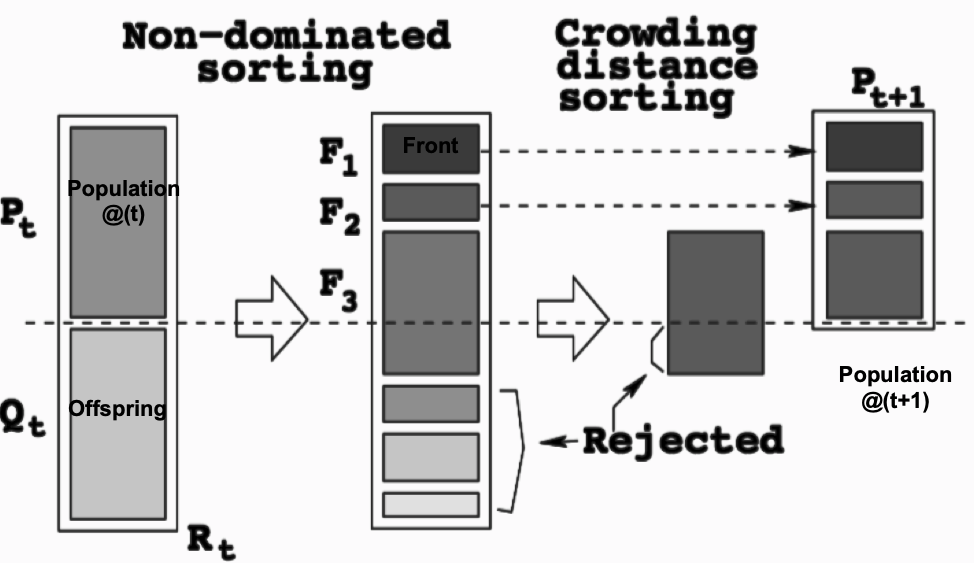
\includegraphics[scale = 0.35]{figs/NSGA_workflow2.png}
    \caption{The NSGA Workflow. At time $t$, an offspring is created through a genetic algorithm~\cite{whitley1994genetic} from an $N-$sized population of design points. 
    The two populations are combined into a population $R_{t}$, which is classified into different non-dominated classes $F_{i}$, starting from the first front $F_{1}$. 
    To restore the initial size of the population, the augmented space of solutions is trimmed. A metric called crowding distance is used to reject solutions and eventually provide an updated population of size $N$ at time $t+1$. 
    Image taken from \cite{deb2002fast}.
    }
    \label{fig:NSGA_workflow}
\end{figure}

Remarkably these approaches can accommodate mechanical and geometrical constraints during the optimization process. In our studies we included at least 5 constraints (\textit{e.g.}, the outermost location of a disk or a layer in the Inner Tracker, or the difference between the outer and inner radius of a disk) during the exploration of the design parameter space.  

A two-level parallelization has been implemented in the MOO framework: the first level creates the parallel simulations of design points, the second level parallelizes each design point. 
The evaluation itself can be distributed to several workers or a whole cluster with libraries like Dask \cite{dask}.


\begin{figure}[!]
    \centering
    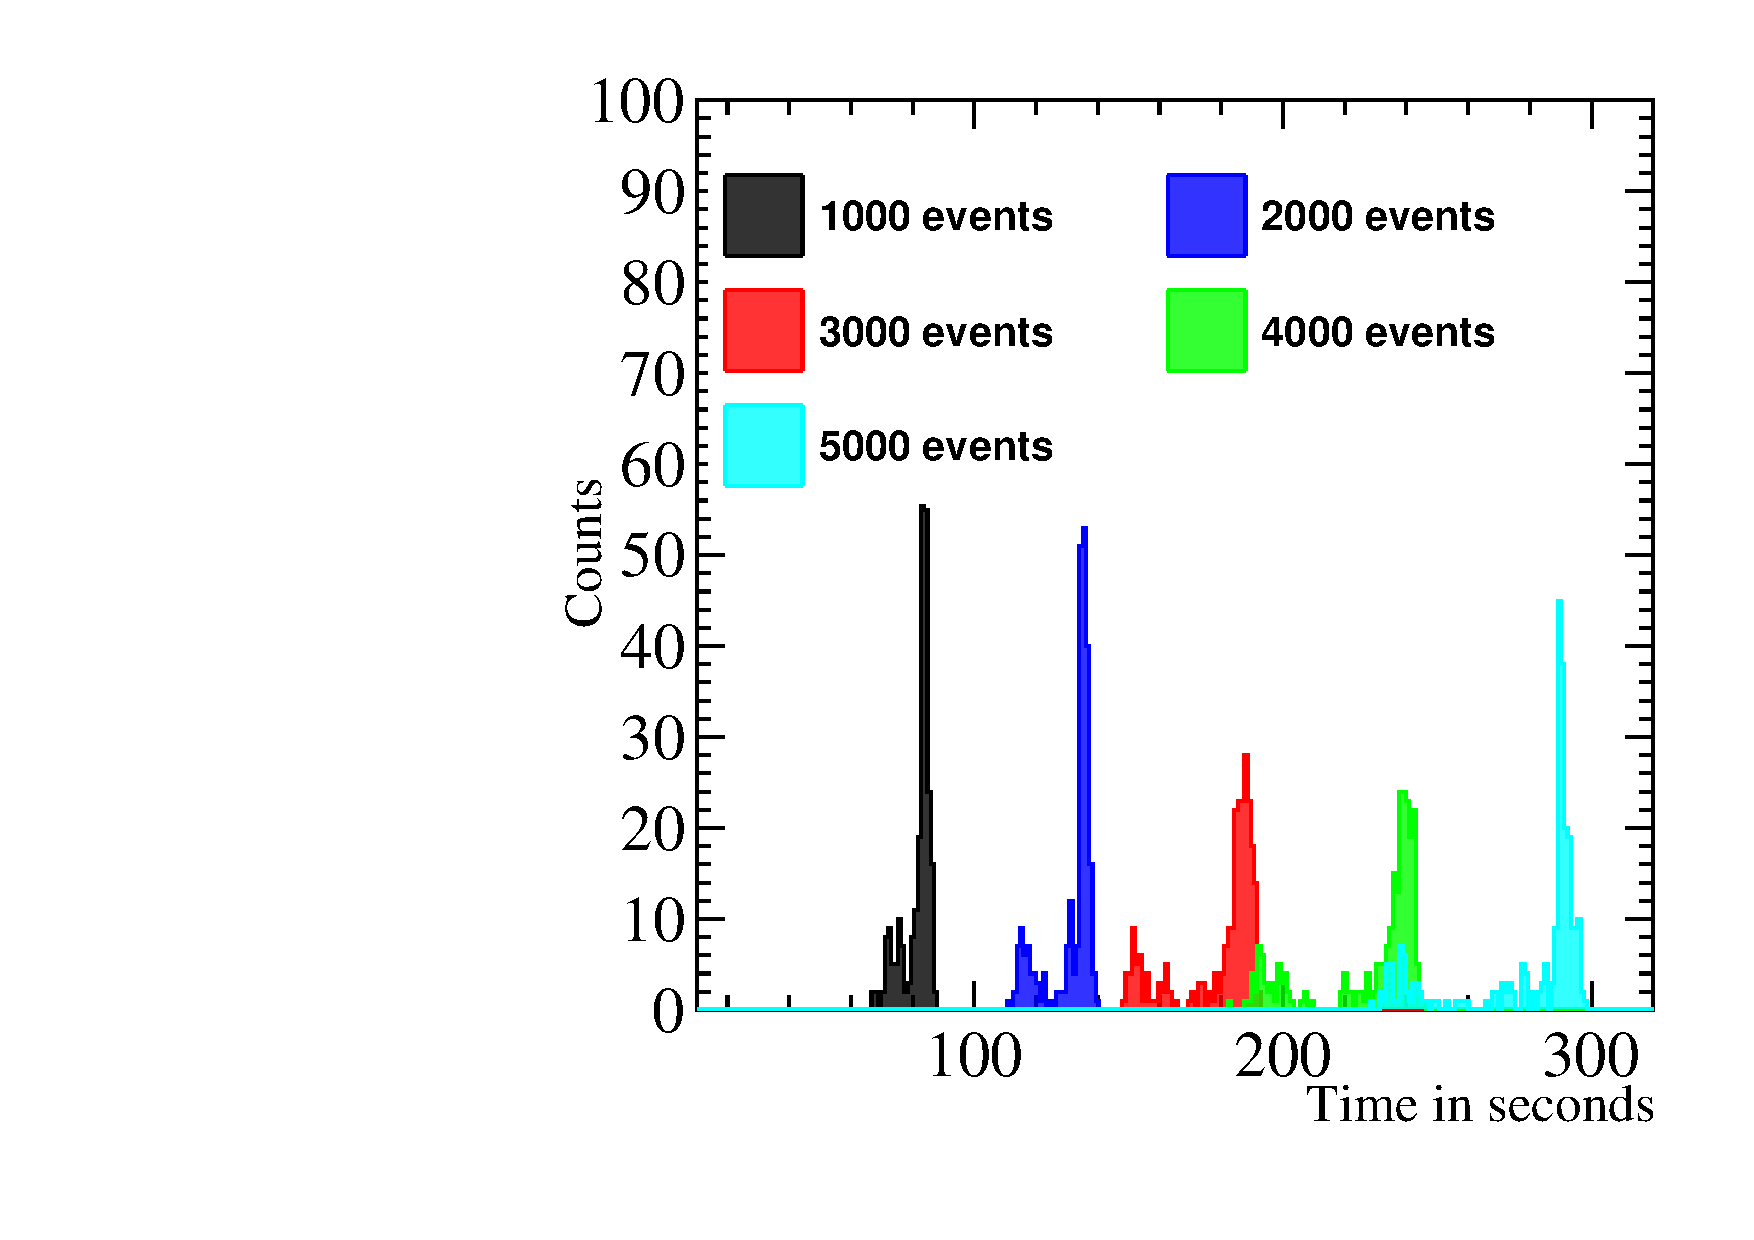
\includegraphics[scale = 0.33]{figs/TimeHistROOT.pdf}
    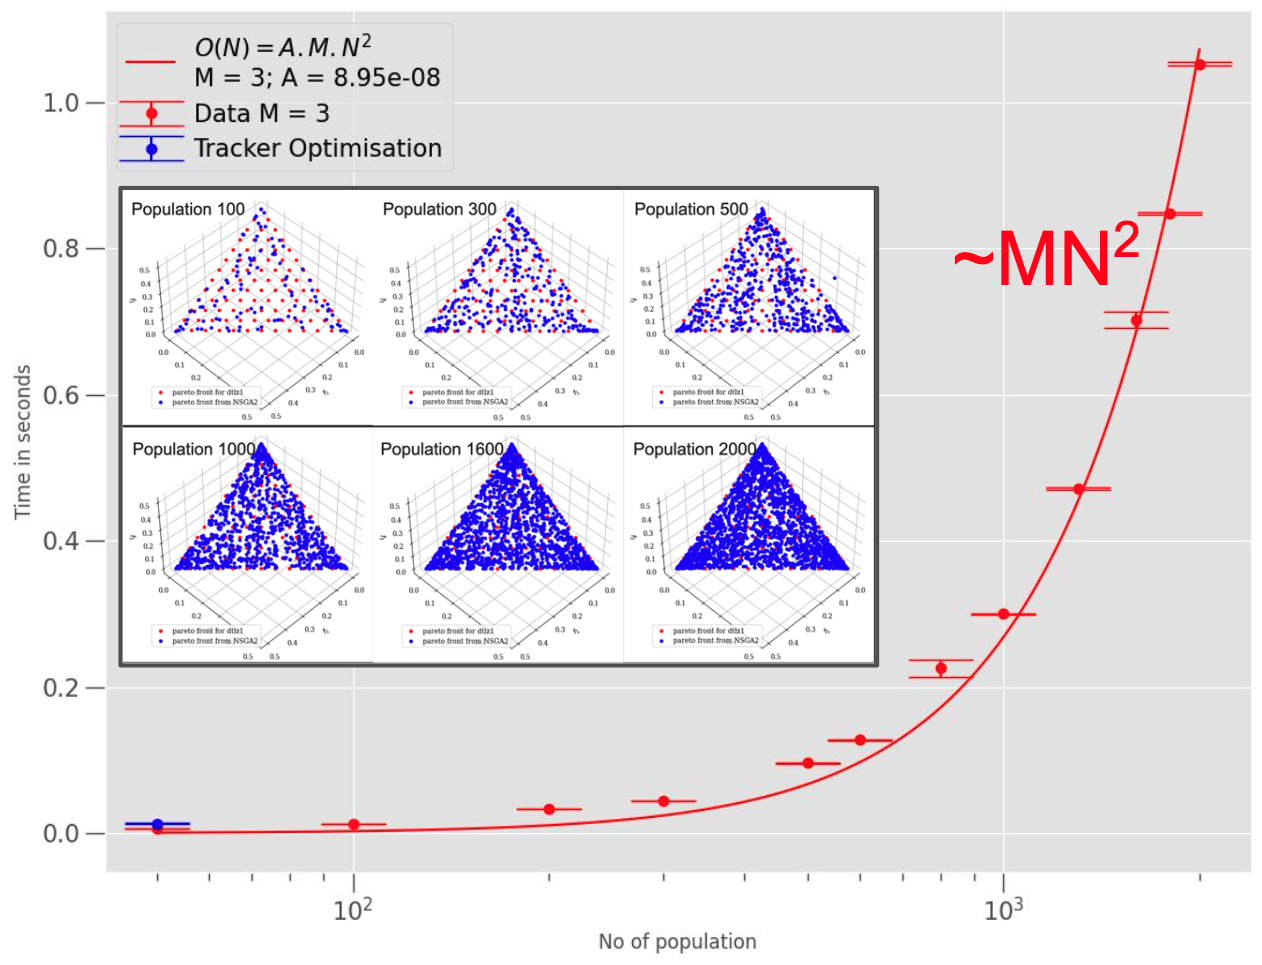
\includegraphics[scale = 0.18]{figs/AI_time_study.png}
    \caption{Computing time studies. (left) The simulation time of a single design point as a function of the number of tracks; (right) the computing time taken by the genetic algorithm and the sorting in NSGA-II. Performance have been benchmark with test problems like DTLZ1 and the scaling $\sim MN^{2}$ has been verified with convergence to the Pareto front. For the complexity of the problem described in Table \ref{tab:complexity}, the simulation time dominates the AI times. A two level parallelization has been introduced in the framework to reduce this bottleneck.  
    The AI contribution typically becomes dominant when very a large population size is needed for an accurate approximation of the Pareto front. 
}
    \label{fig:computing-times}
\end{figure}

AI has played a crucial role in helping to choose a combination of technologies for the inner tracker, as shown in Fig. \ref{fig:improved_with_AI} (top). 
This is a dynamical/iterative process that evolves in time and requires the interplay between the ECCE teams working on Physics, Detector and Computing.
Results are validated by looking at figures of merit that do not enter as objective functions in the optimization process. The decision making is left post hoc and discussed among the Computing, Detector and Physics Teams, see Fig. \ref{fig:improved_with_AI} (bottom).


%The set up framework can be utilized for the optimization of other detectors too.

\begin{figure}[!]
    \centering
    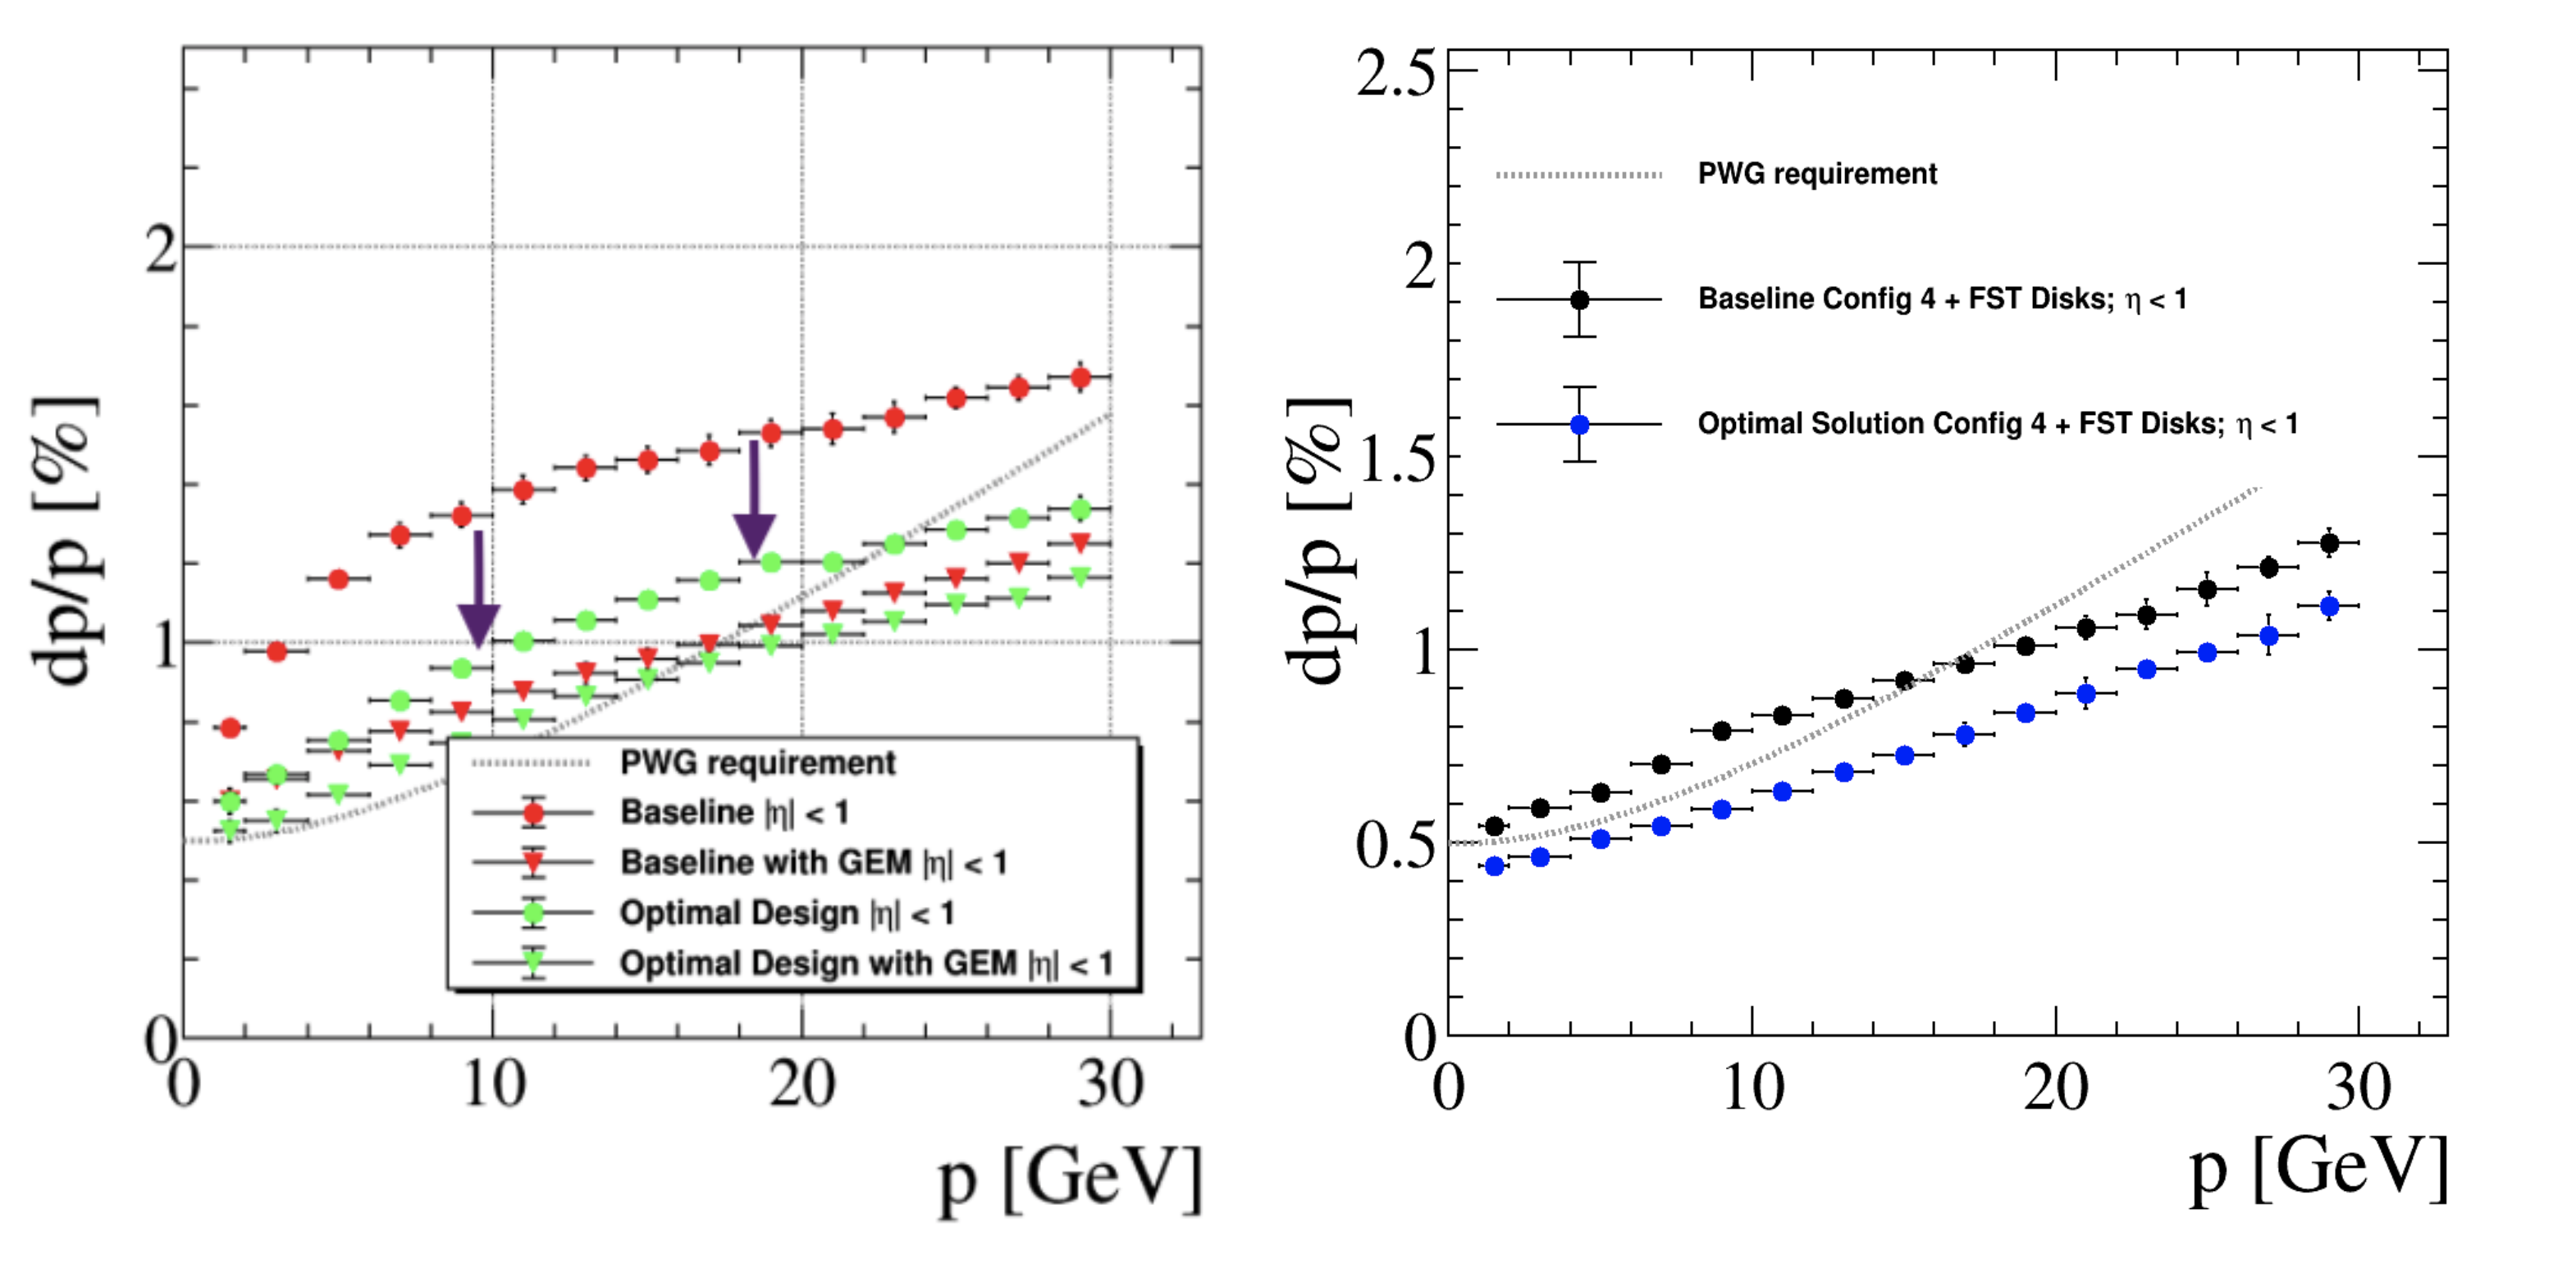
\includegraphics[scale = 0.25]{figs/improve_with_AI.png}
    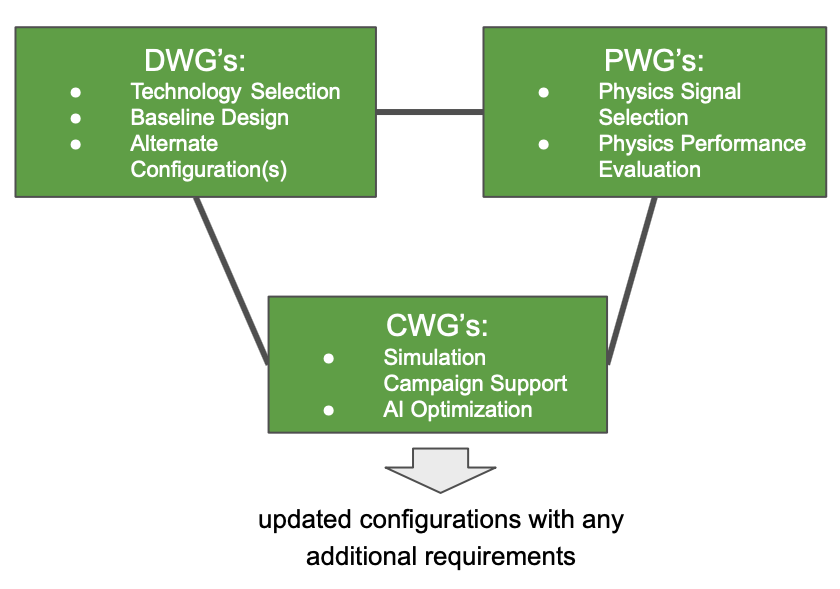
\includegraphics[scale = 0.35]{figs/interplay.png}
    \caption{
    Example of improvement in performance of the Inner Tracker barrel design during the detector proposal ascribable to Artificial Intelligence. AI took the red points (initial design) to green. The detector concept further evolved since then and AI improved it from black to blue by rearranging the geometry and dimensions of the components. It is clear that the fundamental interplay between the ECCE Teams working on Physics, Detector and Computing is propelled by AI in the design process. 
}
    \label{fig:improved_with_AI}
\end{figure}

The reader should be reminded that a Pareto front is potentially made by a set of trade-off solutions. Fig.~\ref{fig:convergence} shows the convergence plot obtained utilizing the hypervolume as metric, and a petal diagram with the three objectives corresponding to one solution in the Pareto front. 

\begin{figure}[!]
    \centering
    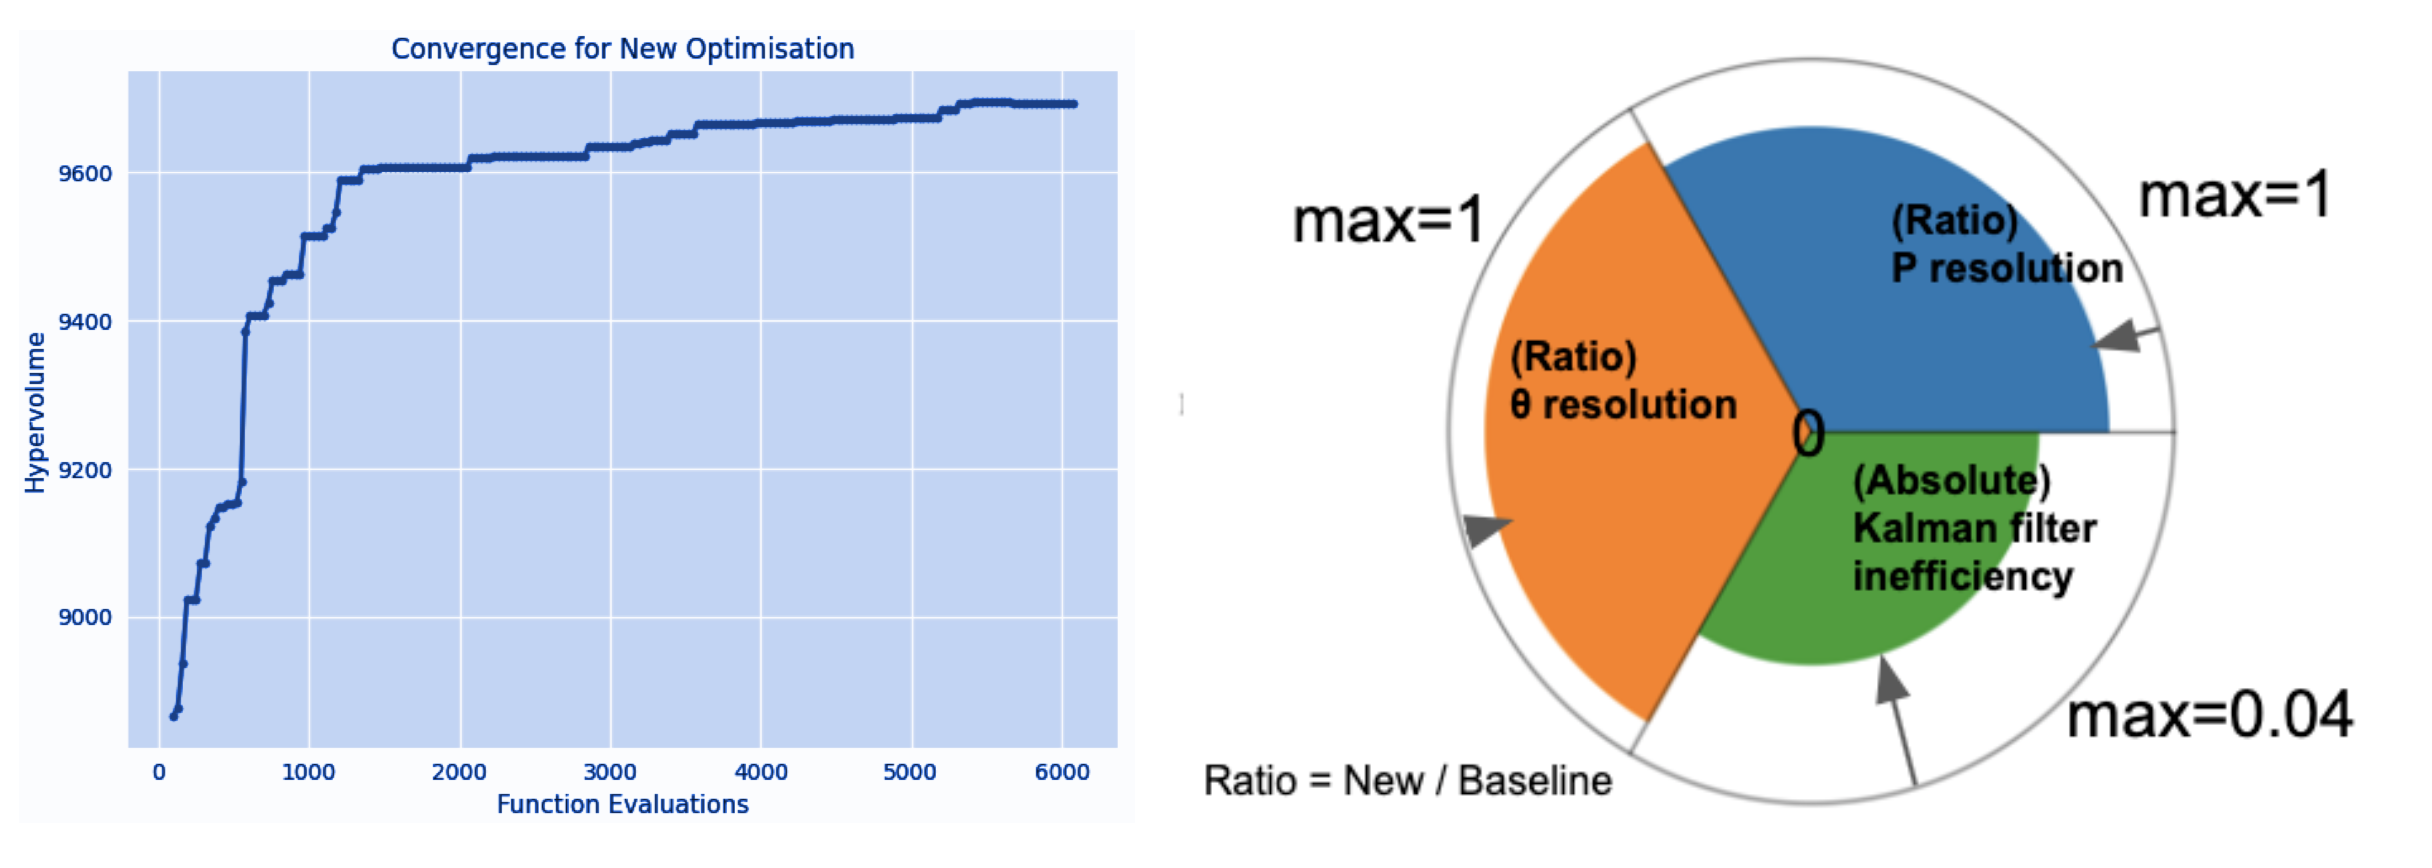
\includegraphics[scale = 0.35]{figs/convergence.png}
    \caption{(left) The hypervolume can be used as a metric for convergence. Checkpoints are created during the optimization and snapshots of the evolving designs can be taken. (right) A petal diagram with the three objectives corresponding to one solution in the Pareto front. The momentum and angular resolutions are expressed as ratios with respect to a baseline design to improve; the KF inefficiency is taken as an absolute value. An optimal design minimizes all of the above defined objectives. 
}
    \label{fig:convergence}
\end{figure}

A complete list of the hyperparameters of our optimization framework can be found in Table \ref{tab:complexity}.
With 11 variables and 3 objectives it has been estimated that about $\sim$10k CPUhours is needed to converge. 


\begin{table}[!]
    \centering
    \begin{tabular}{|M{3.cm} | M{3.5cm}| M{2.0cm}|}
        \hline
        \textbf{description} & \textbf{symbol} & \textbf{value} \\ 
        \hline
        \hline
        \small{population size} & N & 100 \\
        \small{\# objectives}   & M & 3(4)\\ 
        \small{offspring} & O & 30(50)\\
        \small{design size} & D & 11(16) \\
        \small{\# calls (tot. budget)} & $-$ & 200\\
        \small{\# cores} & $-$ & \small{same as offspring} \\
        \small{\# charged $\pi$ tracks} & N$_{\textup{trk}}$ & 80k\\
        \small{\# bins in $\eta$} & N$_{\eta}$ & 3 \\
        \small{\# bins in P} & N$_{\textup{P}}$ & 15 \\
        \hline
    \end{tabular}
    \caption{Summary of the hyperparameters during the optimization. Symbols used throughout the document to describe these quantities are also reported to facilitate the reader. Values not in parentheses correspond to the optimization of a starting reference design. Values in parentheses are the largest ones utilized in other optimization pipelines. Checkpoints are created allowing to take a snapshot of the optimization while ongoing. A survey of the detector performance is created after each call. At each call an offspring of 30 to 50 new design points is created through a genetic algorithm. The framework ran on the JLab computing farm with a maximum number of 128 cores allocated.
    }
    \label{tab:complexity}
\end{table}


%%This approach can be further utilized 
%%We describe our strategy and show preliminary results for the Si tracking system. 

Larger populations of design points can be simulated to improve accuracy of the Pareto front in multidimensional spaces with AI-based accelerated optimizations. 
An interesting trend is scaling the MOO workflows on HPC systems \cite{liu2020parallelization}. 

Remarkably the developed framework can be utilized for other sub-detectors, or systems of sub-detectors.

\clearpage

\section {Online}
\label{sec:online}
%- - - - - - - - - - - - - - - - - - - - - - - - - - - - - - - - - 
\subsection{Data Acquisition}
%\textbf{\emph{Jan B.}}

We envision a DAQ system following a streaming readout paradigm. In the following, we will describe the individual components as well as the overall data flow and bandwidth model. An overview of the system is shown in Figure \ref{fig:data_acquisition_diagram}.


\begin{figure}[hbt!]
 \begin{center}
  % \raisebox{0.5mm}{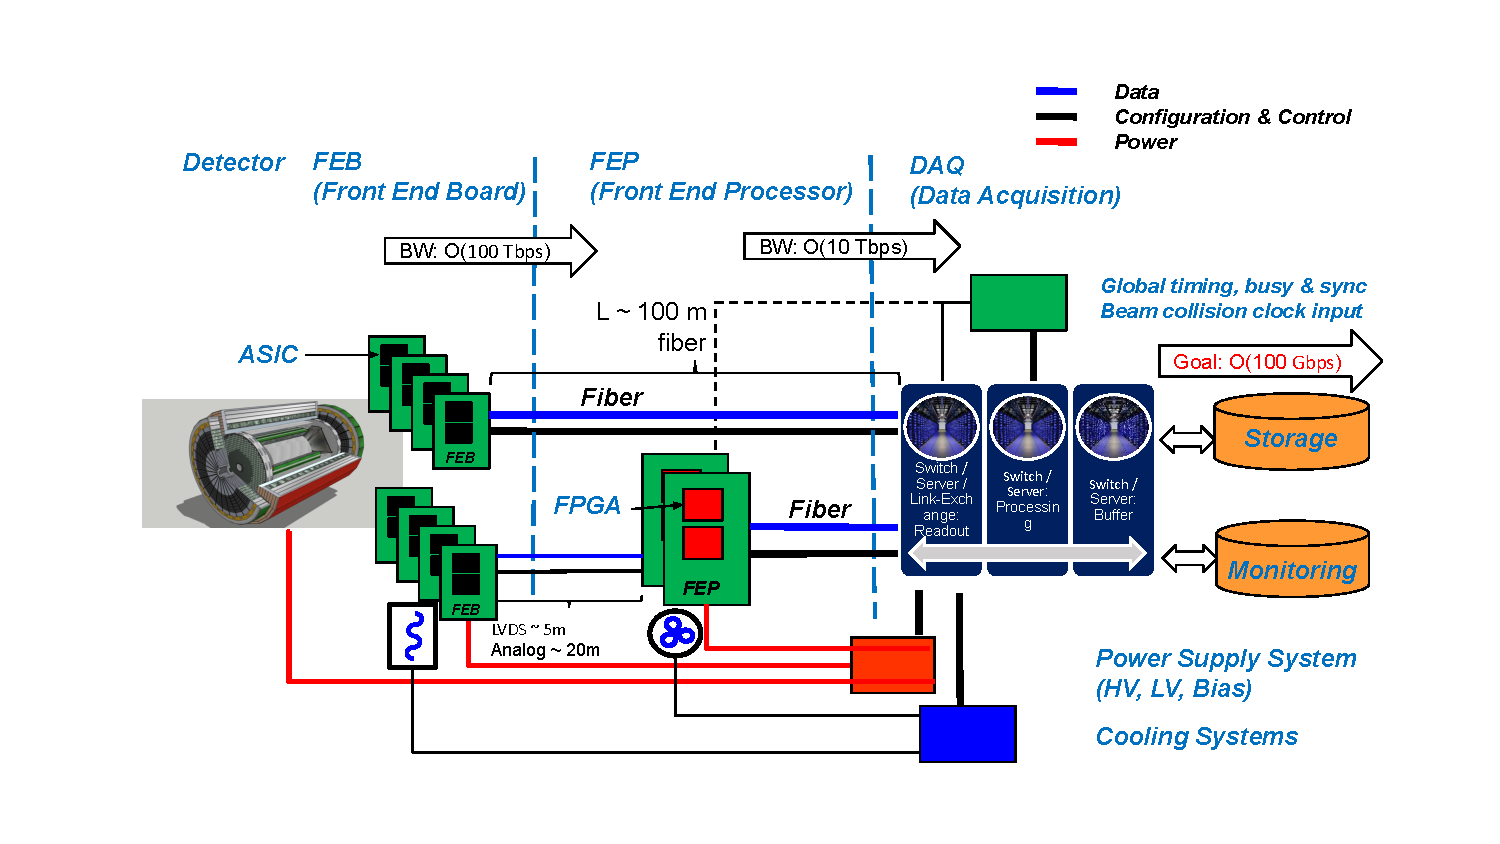
\includegraphics[trim=50 30 50 30, clip, width=0.99\linewidth]{figs/figure_data_acquisition_diagram.pdf}}
  \usetikzlibrary{arrows,chains,shapes,matrix,scopes,positioning,fadings,backgrounds,fit,mindmap,trees,decorations.markings,decorations.pathreplacing,calc}
\usetikzlibrary{decorations.pathmorphing,decorations.markings,trees,arrows.meta}

\definecolor{feeback}{rgb}{0,0.8,0} 
\definecolor{fepback}{rgb}{0,0.8,0} 
\definecolor{fepchip}{rgb}{0,0.9,0.9} 
\definecolor{sagback}{rgb}{0.9,0.9,0} 
\definecolor{sagchip}{rgb}{0,0.9,0.9} 
\definecolor{monitoring}{rgb}{1.,1.,1} 
\definecolor{fibercolor}{rgb}{0.9,0,0} 
\definecolor{locality}{rgb}{0,0.7,0.7} 
\tikzset{   
pics/.cd,   
disc/.style = {    
        code = {    
          \fill [white] ellipse [x radius = 1, y radius = 2/6]; 
     \path [left color = black!50, right color = black!50, middle color = black!25] 
      (-1+.05,-0.55) arc (180:360:1-.05 and 2/6-.05*2/6) -- cycle; 
     \path [top color = black!25, bottom color = white] (0,.05*2/3) ellipse [x radius = 1-.05, y radius = 2/6-.05*2/6]; 
     \path [left color = black!25, right color = black!25,middle color = white] (-1,0) -- (-1,-0.5) arc (180:360:1 and 2/6) -- (1,0) arc (360:180:1 and 2/6); 
     \foreach \r in {225,315} 
       \foreach \i [evaluate = {\s=30;}] in {0,2,...,30}
          \fill [black, fill opacity = 1/50]
             (0,0) -- (\r+\s-\i:1 and 2/6) -- ++(0,-0.5)
             arc (\r+\s-\i:\r-\s+\i:1 and 2/6) -- ++(0,0.5) -- cycle;
      \foreach \r in {45,135}
        \foreach \i [evaluate = {\s=30;}] in {0,2,...,30}
          \fill [black, fill opacity = 1/50]
             (0,0) -- (\r+\s-\i:1 and 2/6)
             arc (\r+\s-\i:\r-\s+\i:1 and 2/6)  -- cycle;
    }   },
  disc bottom/.style = {
    code = { 
     \foreach \i in {0,2,...,30}
        \fill [black, fill opacity = 1/60] (0,-0.55)
          ellipse [x radius = 1+\i/40, y radius = 2/6+\i/60];
      \path pic {disc};
    }   } }
\tikzstyle{vecArrow} = [thick, decoration={markings,mark=at position
   1 with {\arrow[semithick]{open triangle 60}}},
   double distance=3pt, shorten >= 5.5pt,
   preaction = {decorate},
   postaction = {draw,line width=1.4pt, white,shorten >= 4.5pt}]

\tikzstyle{fiber} = [thick, fibercolor]


\tikzset{
fee/.pic ={
	\draw [thick,fill=feeback]  (-0.275,-0.4) rectangle  (0.275,0.35);
	\draw[fill=black] (-0.18,0.25)  rectangle (-0.02,0.15);
	\draw[fill=black] (0.18,0.25)  rectangle (0.02,0.15);
	\draw[fill=black] (-0.18,0.1)  rectangle (-0.02,0.0);
	\draw[fill=black] (0.18,0.1)  rectangle (0.02,0.0);
	\draw (0,-0.2) node{\scriptsize FEE};
},
fep/.pic ={
	\draw [thick,fill=fepback]  (-0.3,-0.4) rectangle  (0.3,0.35);
	\draw[fill=fepchip] (-0.175,0.25)  rectangle (0.175,-0.1);
	\draw (0,-0.25) node{\scriptsize FEP};
},
sag/.pic ={
	\draw [thick,fill=sagback]  (-0.3,-0.4) rectangle  (0.3,0.35);
	\draw[fill=sagchip] (-0.125,0.2)  rectangle (0.125,-0.05);
	\draw (0,-0.25) node{\scriptsize SAG};
},
rack/.pic = {
	\draw [thick,rounded corners=4pt] (-1,2)  rectangle (0.5,-2);
	\draw [thick,rounded corners=2pt] (-0.9,1.9)  rectangle (0.4,1.6);
	\draw [thick,rounded corners=2pt] (-0.9,1.5)  rectangle (0.4,1.2);
	\draw [thick,rounded corners=2pt] (-0.9,1.1)  rectangle (0.4,0.8);
	\draw [thick,rounded corners=2pt] (-0.9,0.7)  rectangle (0.4,0.4);

	\draw [thick,rounded corners=2pt] (-0.9,0.3)  rectangle (0.4,0);
	\draw [thick,rounded corners=2pt] (-0.9,-0.1)  rectangle (0.4,-.4);
	\draw [thick,rounded corners=2pt] (-0.9,-.5)  rectangle (0.4,-0.8);
	\draw [thick,rounded corners=2pt] (-0.9,-0.9)  rectangle (0.4,-1.2);
	\draw [thick,rounded corners=2pt] (-0.9,-1.3)  rectangle (0.4,-1.6);
}, 
smallrack/.pic = {
	\draw [thick,rounded corners=2pt] (-1,2)  rectangle (0.5,-2);
	\draw [thick,rounded corners=1pt] (-0.9,1.9)  rectangle (0.4,1.6);
	\draw [thick,rounded corners=1pt] (-0.9,1.5)  rectangle (0.4,1.2);
	\draw [thick,rounded corners=1pt] (-0.9,1.1)  rectangle (0.4,0.8);
	\draw [thick,rounded corners=1pt] (-0.9,0.7)  rectangle (0.4,0.4);

	\draw [thick,rounded corners=1pt] (-0.9,0.3)  rectangle (0.4,0);
	\draw [thick,rounded corners=1pt] (-0.9,-0.1)  rectangle (0.4,-.4);
	\draw [thick,rounded corners=1pt] (-0.9,-.5)  rectangle (0.4,-0.8);
	\draw [thick,rounded corners=1pt] (-0.9,-0.9)  rectangle (0.4,-1.2);
	\draw [thick,rounded corners=1pt] (-0.9,-1.3)  rectangle (0.4,-1.6);
}, 
rackwfelix/.pic = {
	\draw [thick,rounded corners=4pt] (-1,2)  rectangle (1,-2);
	\draw [thick,rounded corners=2pt] (-0.9,1.9)  rectangle (0.9,1.0);
	\draw (-0.1,1.3) node {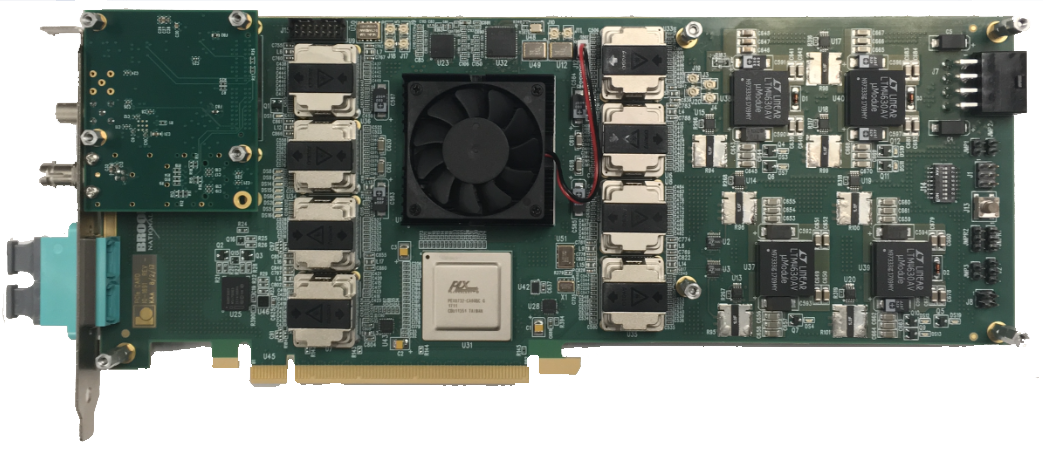
\includegraphics[width=1.5cm]{figs/felix.png}};
	\draw [thick,rounded corners=2pt] (-0.9,0.9)  rectangle (0.9,-0.1);
	\draw (-0.1,0.2) node {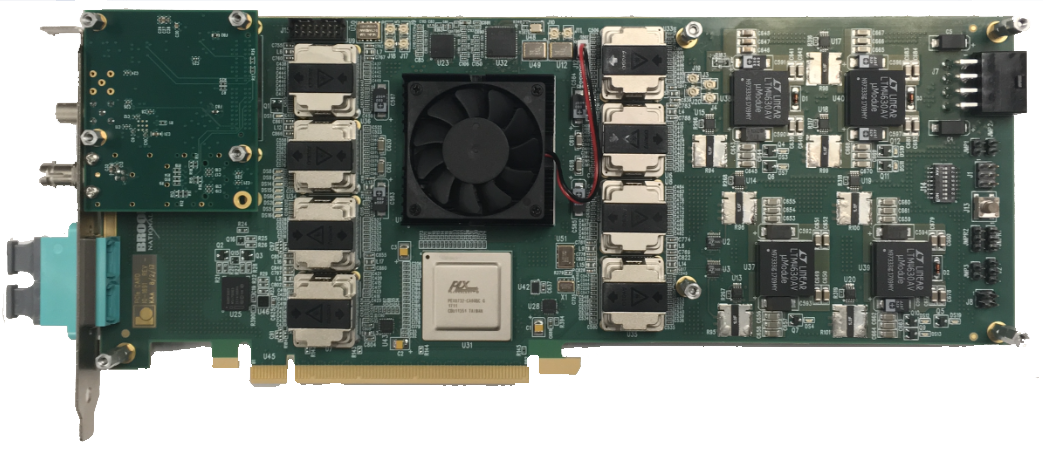
\includegraphics[width=1.5cm]{figs/felix.png}};
	\draw [thick,rounded corners=2pt] (-0.9,-.2)  rectangle (0.9,-1.2);
	\draw (-0.1,-0.9) node {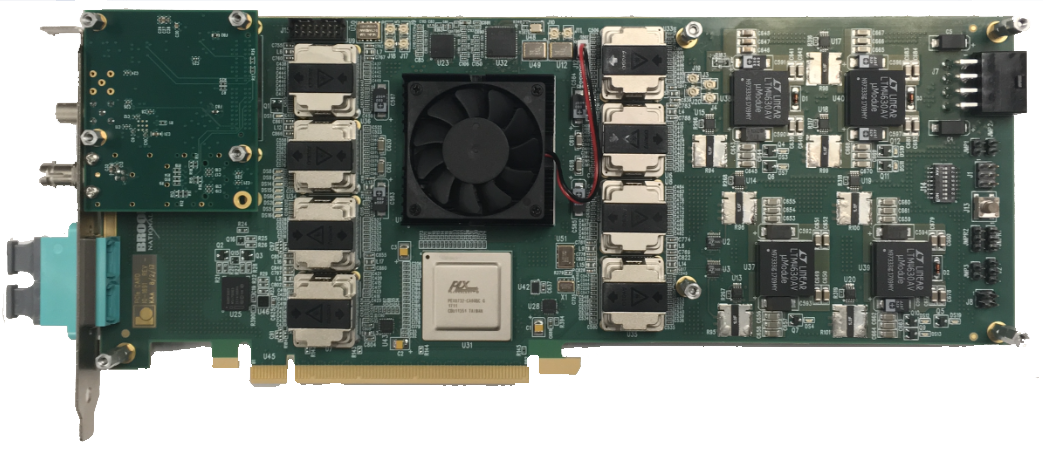
\includegraphics[width=1.5cm]{figs/felix.png}};
	\fill (-0.3,-1.6) circle(0.075);
	\fill (0,-1.6) circle(0.075);
	\fill (0.3,-1.6) circle(0.075);
}
}

{\sffamily
\begin{tikzpicture}     
  \draw (-3,0) node[]{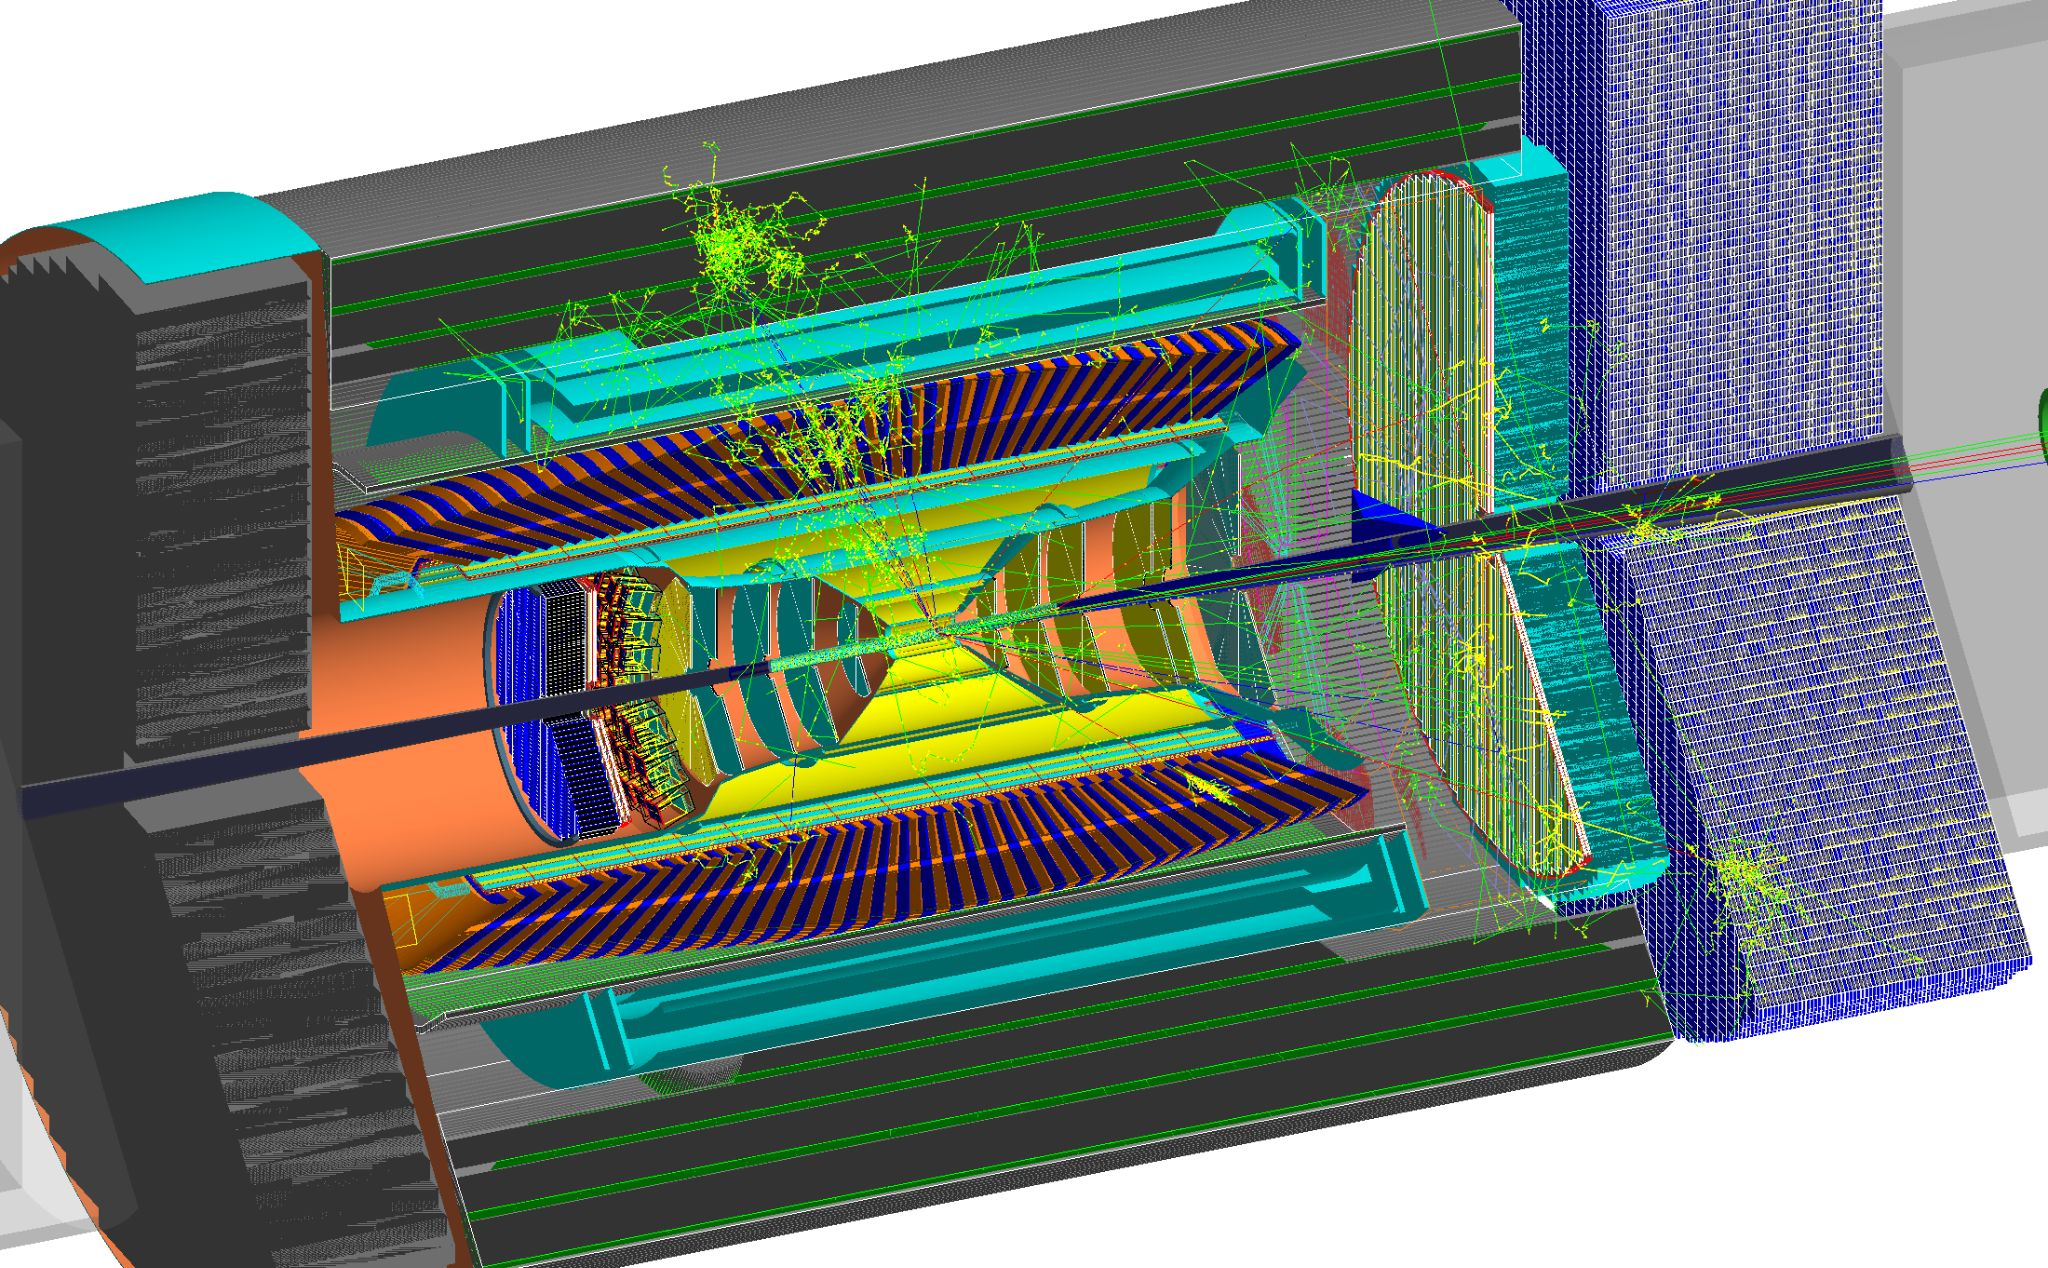
\includegraphics[width=3cm]{figs/detector.jpg}};   

\draw[locality] (-3,3) node {\large Detector};
\draw[locality] (1.5,3) node {\large Exp.~hall};
\draw[locality] (5.9,3) node {\large Counting room};
\draw[locality] (10.2,3) node {\large on-site/off-site};

\draw[locality,dashed,very thick] (-0.3,2.5) -- (-0.3,-5);
\draw[locality,dashed,very thick] (3.3,2.5) -- (3.3,-5);
\draw[locality,dashed,very thick] (8.3,2.5) -- (8.3,-5);



\draw[fiber] (-1.3,1.9) -- (4,1.9);
\draw[fiber] (-1.3,1.7) -- (4,1.7);
\draw[fiber] (-1.3,1.5) -- (4,1.5);
\draw[fiber] (-1.3,1.3) -- (4,1.3);

 \pic at ( -1.6 , 2.0) {fee};
 \pic at ( -1.4 , 1.8) {fee};
 \pic at ( -1.2, 1.6) {fee};
 \pic at ( -1 , 1.4) {fee};


\draw[fiber] (-1.3,0.2) -- (2.3,0.2);
\draw[fiber] (-1.3,0.) -- (2.3,0);
\draw[fiber] (-1.3,-.2) -- (2.3,-0.2);
\draw[fiber] (-1.3,-.4) -- (2.3,-.4);
\draw[fiber] (2.5,-0.1) -- (4,-0.1);
 \pic at ( -1.6 , 0.3) {fee};
 \pic at ( -1.4 , 0.1) {fee};
 \pic at ( -1.2, -0.1) {fee};
 \pic at ( -1 , -0.3) {fee};
  


\draw(-1.3,-1.5) -- (0.3,-1.5);
\draw(-1.3,-1.7) -- (0.3,-1.7);
\draw (-1.3,-1.9) -- (0.3,-1.9);
\draw(-1.3,-2.1) -- (0.3,-2.1);
  
\draw[fiber] (0.7,-1.6) -- (4,-1.6);
 \pic at ( -1.6 , -1.4) {fee};
 \pic at ( -1.4 , -1.6) {fee};
 \pic at ( -1.2,-1.8) {fee};
 \pic at ( -1 , -2) {fee};

\pic at (0.5,-1.75) {fep};

\pic at (2.5,-0.075) {sag};

\pic at (5,0) {rackwfelix};
\pic at (7.1,0) {rack};
\pic[scale=0.5] at (6.75,-3.05) {disc};
\draw  (6.75,-3.4) node[anchor=north]{\small Local buffer};
\draw[thick, rounded corners=3pt,fill=monitoring] (4,-4.6) rectangle (7.75,-5.4);
\draw (5.875,-5.) node {\small Monitoring};


\pic[scale=0.5] at (9.5,-0.6) {disc};
\pic[scale=0.5] at (9.5,-0.3) {disc};
\pic[scale=0.5] at (9.5,0.) {disc};
\pic[scale=0.5] at (9.5,0.3) {disc};
\pic[scale=0.5] at (9.5,0.6) {disc};

\pic[scale=0.5] at (10.75,-0.6) {disc};
\pic[scale=0.5] at (10.75,-0.3) {disc};
\pic[scale=0.5] at (10.75,0.) {disc};
\pic[scale=0.5] at (10.75,0.3) {disc};
\pic[scale=0.5] at (10.75,0.6) {disc};



\draw[implies-implies,double distance=0.15cm] (7.7,-0.1) -- (8.9,-0.1);

\draw[implies-implies,double distance=0.15cm] (6.75,-2) -- (6.75,-2.85);

\draw[-implies,double distance=0.15cm] (6.75,-3.9) -- (6.75,-4.6);
\draw[-implies,double distance=0.15cm] (5.0,-2.1) -- (5.0,-4.6);


\draw (1,2.1) node {\small Fiber};
\draw(-0.5,-2.7) node {\small LVDS $\mathcal{O}$(5)m};
\draw(-0.5,-3.1 ) node {\small analog $\mathcal{O}$(20)m};

\pic[scale=0.5] at (9.5,-3.5) {smallrack};
\pic[scale=0.5] at (10.5,-3.5) {smallrack};
\pic[scale=0.5] at (11.5,-3.5) {smallrack};

\draw[implies-implies,double distance=0.15cm] (9.5,-1.1) --(9.5,-2.4);
\draw[implies-implies,double distance=0.15cm] (10.75,-1.1) --(10.75,-2.4);
\draw (10.5,-5) node{\small  JLAB,SDCC, OSG, ...};

\end{tikzpicture}
}
  
  \caption[Data Acquisition Diagram]{\label{fig:data_acquisition_diagram} The DAQ electronics deployment can be roughly divided by their location, with Front End Electronics (FEE) modules on/near the detector, data aggregators in the hall, and online filtering and monitoring in the counting room. Long term storage and analysis processing is performed in a federated model on multiple sites. }
  %\caption[Data Acquisition Diagram]{\label{fig:data_acquisition_diagram} Diagram of a Data Acquisition system. This is reproduced from slides shown at AI4EIC 2021\cite{EIC_readout_overview_AI4EIC_2021}. }
 \end{center}
\end{figure}


\subsection{DAQ components}
 Front-end electronics (FEE) modules sit inside or on the detector. In most cases, detector-specifc ASICs provide the data conversion from the analog to digital domain, do zero-suppression and provide an interface to fiber transceivers for data transport to the counting room.  There, we envision FELIX-type PCIe-based receiver cards\footnote{In the following, we will use "FELIX card" as a stand-in for a successor board of similar architecture.} which support a large number of high speed fiber links per card.  

Since some FEE may not utilize the full bandwidth of a fiber link, cost-effective stream aggregator boards (SAGs), based either on small FPGAs or COTS multiplexer ICs, can bundle multiple fiber links coming from FEE to a single fiber to the FELIX cards. 

Because of space and services constraints, or because no suitable ASIC is available, some FEEs will connect to Front end processor (FEP) modules via digital (LVDS) or analog links. The FPGA and possibly analog to digital converter logic on the FEP will then generate a data stream suitable for fiber transport to the FELIX cards.

In the counting room, we expect a number of special servers which house the FELIX cards. Each FELIX/CPU combination sees data from a certain subset of detector channels and can do additional data reduction before sending out the data to the counting room CPU farm. This CPU farm (with possibly GPU accelerators) will do further data reduction, for example via high level data selection algorithms.

The data streams are buffered on local hard disks, with enough capacity to store the data for several days. This local buffer has multiple functions: 
\begin{itemize}
    \item It averages out the changes in data rate from luminosity changes so that the upstream link only need to provide average, not peak, bandwidth.
    \item It allows stand-alone operation for a limited time when the data transport out of the counting house is not available or runs at reduced capacity.
    \item It allows for near-online monitoring and replay of recent data for quality control, especially for those quantities which depend on on-going calibrations.        
\end{itemize}

The data are then pushed upstream to on-site or federated storage as part of the overall EIC project.


\subsection{Online monitoring}
Online monitoring is divided into a fast path with bound latency and a slow path. The former path supports the requirements for accelerator steering and equipment protection with regards to possible reaction time. The data is either generated on the FELIX host CPUs or on the FELIX card themselves. Necessarily, they are limited in scope to counting, summing or similar type of information. The slow path provides higher-level information for quality control. Here, its is possible to reconstruct and analyse full events on-the-fly, by copying pre-selected time segments from the data stream to the analysis sub-cluster. Note here that such a monitoring system does not require the guaranteed reconstruction of all data, just of a suitable subset. That subset can either be selected unbiased by selecting periodic time segments, or biased by selecting time-segments tagged by data filters in the main data stream.  Similar monitoring can be performed on data on the local buffer for those quantities which require calibration data or two-pass analysis.

% DL
For both types of data a system will be needed to evaluate the monitoring data and inform the experiment operators of potential issues. This will largely include the creation of histograms which may be monitored either graphically or by some automated means. The prevalence of AI will certainly play a large role in that it will be able to evaluate a wider variation of monitoring data and at a much higher rate than could be expected of humans. Such systems are already deployed and under development~\cite{Hydra2021}. 

\subsection{Risk mitigation}
We expect that during initial commissioning noise rates will be significantly higher than during established operation, as accelerator and detector parameters will not yet be tuned optimally. Such high noise rates might overwhelm processing and upstream write capability. To allow progress in this initial phase, the DAQ system will allow to input a bounded-latency signal on the FELIX card or host CPU level to suppress uninteresting time segments.

Such a system also allows us to simply incorporate a dedicated collision detector for rate reduction: only time segments which are flagged to have a collision are kept, others are dropped early in the processing chain. 

This bounded-latency system could either be realized as a classic electrical trigger signal, or via software messages sent to the FELIX hosts with a clear advantage with regard to flexibility and ease of implementation, but with possibly a larger latency. The optimal implementation depends on the capabilities of the future FELIX successor and bandwidth availability on the FELIX host servers.

\subsection{Expected data rates and reduction steps}

%\emph{JCB: I'm not sure how valid these numbers are.}

Since connections between detector and FEPs might not be zero-suppressed digital or even analog data, it makes no sense to specify a data rate at the detector-to-hall border. Instead, the following section describes the expected data rate on the Fiber/FELIX level and downstream from there.

At nominal luminosity, we expect that true signals and beam-gas interactions produce a total rate of $\mathcal{O}$(100 Tbps) of zero-suppressed data at the FELIX card level. However, detector noise and additional backgrounds, especially during early operation, can completely dominate this rate. We assume therefore a total rate of $\mathcal{O}$(10 Tbps) bandwidth on the fiber level. Next-gen FELIX cards will have 25 GBps receivers, for headroom for burst rates, non-ideal allocation of detector channels to fibers \emph{etc.}, we assume 12.5 GBps as the average rate per fiber, and as a consequence, about 800 fibers.

A current-generation FELIX card has 48 fiber ports, leading to $\mathcal{O}$(20) FELIX cards. Each card would then receive 600 GBps. We assume that at the time of procurement for EIC, cards with at least PCIe Gen5 are available, providing 500 GBps to the host server, requiring a modest reduction of the data rate in FELIX card itself, for example via cross-channel noise reduction. In combination with the host CPU, we expect a total reduction by a factor of 5 to $\mathcal{O}$(2) Tbps total, 100 GBps per server. We note that a typical server with 128GB of memory can buffer the full stream for about 2 seconds, ample time for region-of-interest/time-slice-of-interest communication between the FELIX hosts, making higher reduction factors likely. The data can then be streamed out via a dual 100 Gbps link to the second layer in the compute farm.

In the compute farm, the data is further analyzed and filtered. We expect that with inter-detector noise suppression and high-level data selection the required effective bandwidth to long-term storage can be reduced to $\mathcal{O}$(100) Gbps.  



%--------------------------------------------------------------------






\section {Offline}
\label{sec:offline}

\textbf{\emph{David L.}}

Offline software encompasses many aspects of the experiment. This includes a number of systems, each of which requires either new development or implementation of existing systems using dedicated experts(s). These include:

\begin{itemize}
    \item Calibration system and database
    \item Reconstruction framework
    \item Reconstruction algorithms
    \item Simulation
    \item Offline Monitoring system
    \item Reconstruction workflow (HPC/HTC job management)
\end{itemize}

In the following sections we describe some of these that will constitute larger efforts in terms of person-hours. It should be noted that at this time certain technology choices seem likely (e.g. GEANT4~\cite{ALLISON2016186}). However, others such as the choice of database systems, file formats, and software frameworks are purposefully left unspecified at this point in time.

%- - - - - - - - - - - - - - - - - - - - - - - - - - - - - - - - - 
\subsection{Reconstruction}

\textbf{\emph{Joe O.}}

In the past several decades, many reconstruction frameworks have been developed by different experiments within both HEP and NP. Several features stand out as common to all of these, which the ECCE software framework must utilize. The most important of these are modularity and user friendliness, as any large HEP/NP collaboration will necessarily comprise many hundreds of scientists with varying levels of software expertise. Therefore, these, and other generic features of excellent software, will be essential. It will additionally be imperative to recognize that software technologies change rapidly, and the ability for the software ecosystem to pivot with ease will be essential. As an example, while \texttt{git} is the de facto modern standard for code versioning and storage, it is impossible to say what versioning technologies will exist ten or more years from now when the EIC will be taking data. ECCE has not committed itself to a particular software ecosystem yet; however, these discussions will need to begin in early 2022 as these decisions will need to be made in preparation for development of a TDR.

One of the trademarks of excellent reconstruction software is reproducibility. ECCE will archive several daily builds that will provide users with the latest snapshot of the software; additionally, weekly builds that persist for longer periods of time will allow tracking of code evolution. In conjunction, special tagged production builds will be archived for large centrally produced data samples, such as those that were produced in preparation for the ECCE proposal. Currently the tagged releases are performed based only on time (e.g. weekly builds). Future software versions will consider implementing modern versioning practices such as semantic versioning~\cite{semantic}. In addition to archived builds, continuous integration is another tool ensuring reproducibility. ECCE does not currently deploy robust continuous integration; however, automated tools enabled by services such as Jenkins or GitLab Runners will be deployed utilizing code checking tools and benchmark analyses. 

Making software user friendly requires that it is distributed in a convenient way. Currently the ECCE framework is distributed with \texttt{cvmfs}, a package managing software developed at CERN~\cite{cernvm}, while the software environment is containerized and deployed with Singularity~\cite{singularity}. Any software system that ECCE decides on will necessitate these tools for distribution, to ensure that all users can easily access the software and that a reproducible environment is available when deploying offline analysis and simulation in a federated computing architecture.

The role of hybrid architectures should also be considered in the ECCE reconstruction framework. Specifically, the use of GPU architectures will be important both for integrating machine learning into reconstruction workflows as well as generically taking advantage of the significant computational speed improvements that GPUs can provide. This integration has the added benefit of potentially utilizing the various leadership computing facilities that are available at national laboratories around the country, for more see Section~\ref{sec:offsite}.


Based on the experience of other experiments, reconstruction software should also take advantage of common software projects that are deployed across the world. For example, the A Common Tracking Software (ACTS) package, initially designed for use at the HL-LHC, has been implemented into the sPHENIX track reconstruction framework~\cite{Osborn:2021zlr}. Several collider-physics-based open source projects exist within the broader HEP community and have recently grown in in their user base, examples include ACTS~\cite{Ai:2021ghi}, Rucio~\cite{Barisits:2019fyl}, PanDA, Fun4All~\cite{fun4allGithub}, Gaudi~\cite{Gaudi}, and others. These should be evaluated for use within the ECCE software stack in early 2022 as a part of the decision making process for the future of the offline software framework.

%\emph{This section should focus on the features that are needed for the reconstruction framework. This should avoid committing to a particular software package at the moment. That is a discussion/decision we should have in early 2022 and I think this section can state that explicitly. Features that will be needed should be driven by HTC system requirements. Specifically, the ability to parallelize both vertically and horizontally. Use of heterogeneous hardware. Containerization and distribution(e.g. CVMFS) should also be discussed. Another general issue is how to distribute calibration and meta-data to potentially 100k jobs without them all hitting a single central server at once. Provisioning for multiple, replicated servers would be appropriate here.}

%\emph{This will need standard statements about modularity and user friendliness of the framework. I think it would be safe to state that we expect the primary language to be C++ while not excluding the integration of other languages.}

\emph{Need estimates of total CPU}

%- - - - - - - - - - - - - - - - - - - - - - - - - - - - - - - - - 
\subsection{Calibration}

\textbf{\emph{Jin H.}}

\emph{The calibration system will be integrated into the Online/DAQ with the goal being to to produce calibrations in ``real time'' a'la LHCb. This should give some details included expected latency/disk space, etc.}

\emph{Another important aspect will be how the calibration DB identifies chunks of time. We discussed making boundaries at lumi blocks corresponding to electron beam fills that are expected to happen at about 1Hz.}

\emph{Need estimate of size of calibration DB/year of operation. This will be small compared to raw data, but since it will be maintained by different machines and software, it is worth breaking out.}

%- - - - - - - - - - - - - - - - - - - - - - - - - - - - - - - - - 
\subsection{Simulation}

\textbf{\emph{Cameron D.}}

\emph{Assume simulation will be done with GEANT4. Work is starting that will implement task-level parallelism to GEANT4 with support for GPUs (Makoto Asai). Should we build in multiple major development cycles to allow us to incorporate these new features as they become available?}

\emph{Open questions include:}
\begin{itemize}
    \item \emph{Geometry definition and versioning}
    \item \emph{Integration of Simulation and Reconstruction software}
\end{itemize}

\emph{Discuss global campaigns and support for local simulations by collaboration members.}

\emph{Need estimates on amount of CPU/GPU needed for simulation per year. }


\section {Offsite Processing}
\label{sec:offsite}


The EIC will be a large international project with many researchers and stakeholders spread throughout the globe. While the accelerator and detectors are necessarily placed at a single locale, the computing need not be and can better reflect the geographic diversity of the collaborations involved in EIC research. In the modern age, high speed network connectivity has become very robust. In the time frame of the EIC ($\sim 2030$) we can expect even more reliable and even faster networks. This will make transporting data on the scale the EIC is expected to produce fairly routine. To give specific numbers, BNL has a 400Gbps connection to the ESnet backbone in 2021. ECCE is currently estimated to produce 100Gbps of raw data once it is in full production sometime around 2030. Network bandwidths have shown steady growth of about 50\% per year over the past few decades\cite{nielsensLaw2019}. Thus, over the next 8 years we can expect existing bandwidths to grow by roughly a factor of 25. Even a conservative estimate that the BNL external connection bandwidth grows by only a factor of 10 means the entire ECCE raw data volume can be streamed out using only a few percent of the total available bandwidth.

This section will briefly describe how a federated computing model for the EIC might look, how it will be used to process the raw data, and how it will also be used to process the large amounts of simulation needed for the program.

%-------------------------------------------------------------------
\subsection{Federated computing}

EIC data processing will employ a federated computing model where multiple facilities will be used. A similar strategy has been successfully deployed by the LHC in the form of the Worldwide LHC Computing Grid (WLCG) or simply \emph{the Grid}\cite{SHIERS2007219}. The benefits of distributing the computing across multiple sites include:

\begin{itemize}
    \item Each site only needs to handle a fraction of data
    \item EIC computing becomes a smaller fraction of each compute farm
    \item One site having diminished capacity temporarily can easily be absorbed by others without reconfiguration
\end{itemize}

Generally speaking, diversifying helps to mitigate certain risks. 

The WLCG model of the LHC is based on multiple \emph{Tiers}, structured in a pyramid type fashion. The topmost tier (\emph{Tier 0})represents the LHC/CERN where the data is produced and all data is stored. It also supplies around 20\% of the total computing resource and does the initial reconstruction of the data before distributing it to the Tier 1 sites\cite{WLCG_Tiers_website}. The Tier 1 sites perform large scale reprocessing of the data and distribution to the Tier 2 sites. The Tier 2 sites do more specialized analysis and simulations while the Tier 3 sites are end users. Each tier in the system only communicates with tiers directly above or below it in the hierarchy.

For the EIC one may consider an alternative model in which the data producer (the experiments of the EIC) and the BNL compute facility (e.g. SDCC) are independent. This allows computing at BNL to become part of a pool of facilities that handle the computing as a federated resource. Figure \ref{fig:federated_offsite_butterfly} illustrates such a model referred to here as a ``\emph{Butterfly}'' model due to the rough shape of the figure. In this model, both compute and storage are distributed with the storage being focused in the Echelon 1 sites. This means access to the data by the end users will be done by connecting Echelon 3 sites directly to Echelon 1 sites. The Echelon 1 sites will themselves provide significant compute capability, but may also farm out large campaigns to Echelon 2 sites. In the simulation campaigns performed for the ECCE proposal, the model shown in Fig.~\ref{fig:federated_offsite_butterfly} was successfully implemented for simulated data production.

\begin{figure}[hbt!]
 \begin{center}
   \raisebox{0.5mm}{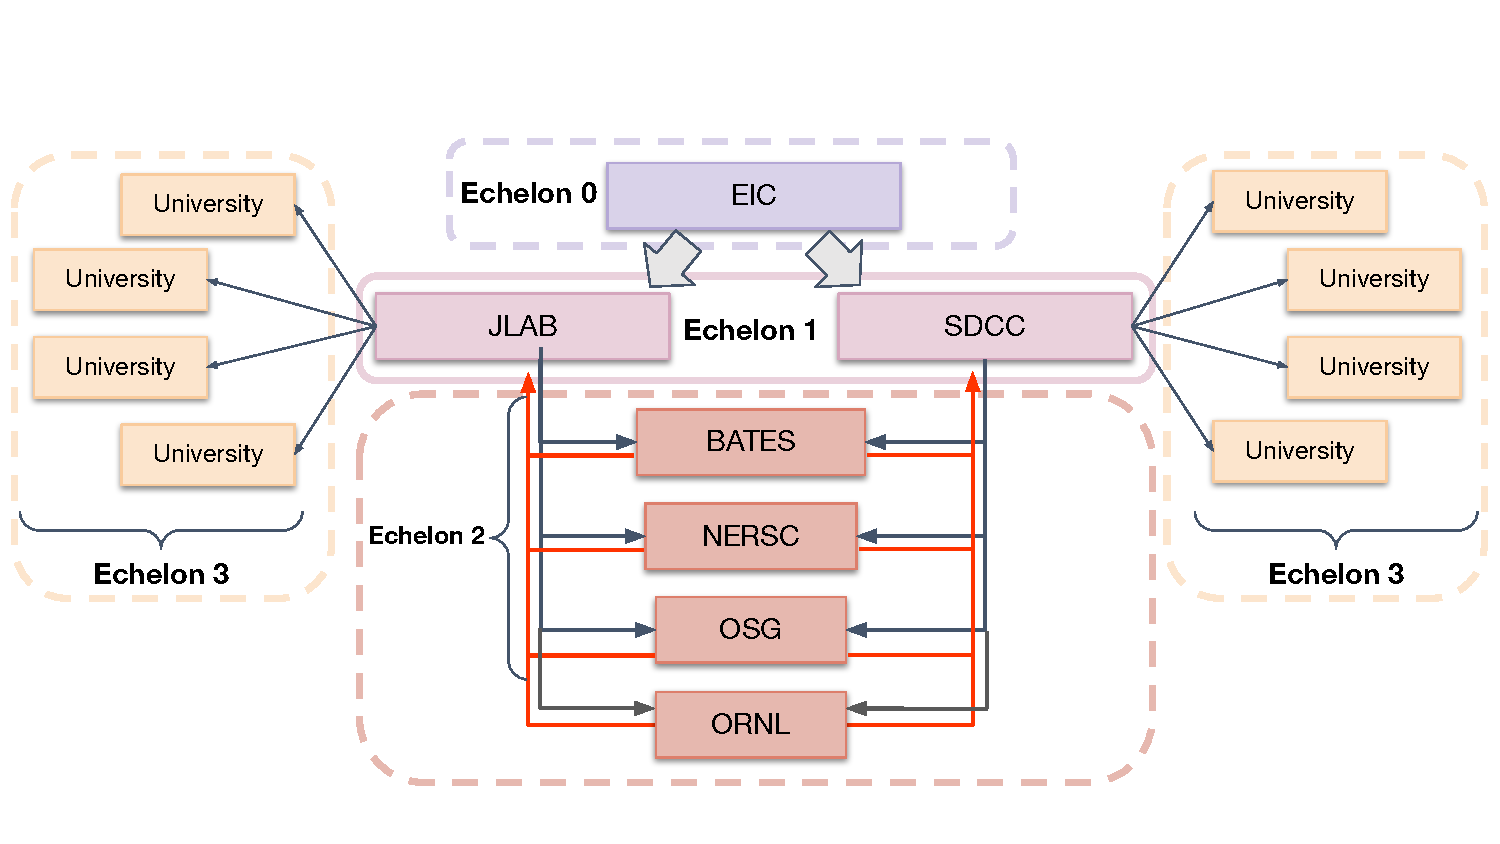
\includegraphics[clip, width=0.99\linewidth]{figs/computing_figure_federated_offsite_butterfly.pdf}}
  \caption[Federated Computing Butterfly model.]{\label{fig:federated_offsite_butterfly} Butterfly model of federated offsite computing. In this model, nearly all storage is contained in echelon 1 while large portions of the raw data processing is delegated to multiple HTC/HPC facilities. The named facilities in this graphic are merely examples and do not represent commitments or final plans.}
 \end{center}
\end{figure}

%-------------------------------------------------------------------
\subsection{Raw data compute}
Processing of EIC data will occur over multiple sites which will include HTC facilities at both BNL and JLab and possibly others. The plan calls for processing the raw data into reconstructed objects such as tracks, jets, and calorimeter clusters within 2-3 weeks of acquisition. The bulk of the few week latency will be due to the time it takes to calibrate the data so that reconstruction may occur. Figure \ref{fig:federated_offsite_example} illustrates how such a scheme could work. The raw data read from the streaming DAQ system will need to be reduced over multiple filtering and compression stages to a rate that is reasonable to transport offsite from BNL using its external network connection. Table \ref{tab:reduction_factors} lists the stages and with in-going and out-going rates and their respective reduction factors. Potential technologies that could be applied at each stage are also listed.

The DOE lab systems are connected via the ESNet unclassified network for scientific research~\cite{ESNet}. As of 2021, BNL has a 400Gbps connection to ESNet and JLab has dual 10Gbps connections. In 2022 or 2023, JLab is anticipated to increase its bandwidth to at least 100Gbps. When the EIC begins collecting data around 2030, one may expect a 1Tbps bandwidth between the two labs. This is an order of magnitude higher than the anticipated raw data rate after filtering from the ECCE detector. Thus, transfer of the entire raw data set offsite from BNL in 2030 seems reasonable.


\begin{figure}[hbt!]
 \begin{center}
   \raisebox{0.5mm}{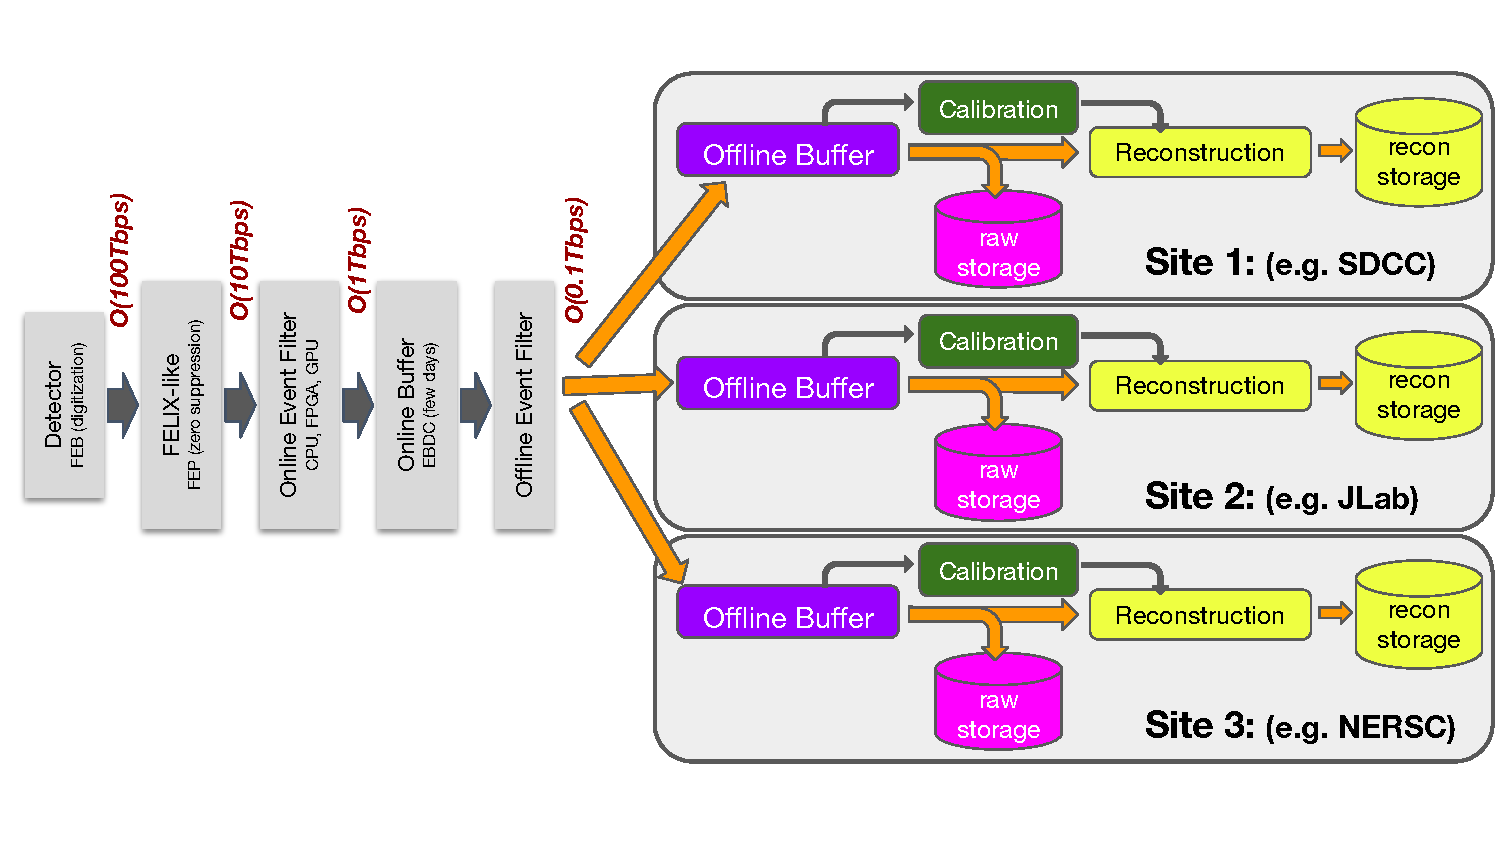
\includegraphics[clip, width=0.99\linewidth]{figs/figure_federated_offsite_example.pdf}}
  \caption[Example of federated processing of data in near real-time using multiple sites.]{\label{fig:federated_offsite_example} Data flow from detector to reconstructed object files (left to right). This diagram illustrates how raw data may be distributed to multiple sites in near-real time. On the left side of the plot, multiple filter and buffering stages are used to reduce the data rate. On the right, the data is distributed to multiple facilities.
  Each facility would store a portion of the raw data. It would also need to keep the data live (e.g. on disk) long enough for it to be calibrated and then processed by the reconstruction software.}
 \end{center}
\end{figure}

\begin{table*}[ht]
    \centering
    \begin{tabular}{p{4cm}|c|c|c}
        \hline
        Stage                        & Input/Output    & Reduction Factor & Technology options \\
        \hline
        \hline
        Compute Interface (e.g. FELIX) & 100Tbps/10Tbps  & $\times 10^{-1}$ & FPGA \\
        \hline
        Online Event Filter          & 10Tbps/1Tbps    & $\times 10^{-1}$ & FPGA, (GPU), CPU\\
        \hline
        Online Buffer                & 1Tbps/0.5Tbps   & $\times 5x10^{-1}$  & $<disk>$ \\
        \hline
        Offline Event Filter         & 0.5Tbps/100Gbps & $\times 2x10^{-1}$  & FPGA, GPU, CPU \\
        \hline
        Reconstruction               & 100Gbps/10Gbps  & $\times 10^{-1}$ & (FPGA), GPU,CPU\\
        \hline
        \hline
        \textbf{Total}               & \textbf{100Tbps/10Gbps} & \textbf{$\times 10^{-4}$} & \\
        \hline
    \end{tabular}
    \caption{Data rates and reduction factors for proposed near real time data flow. Estimated data rate from ECCE detector is $\mathcal{O}(100Tbps)$. Raw storage will be $\mathcal{O}(100Gbps)$. Reconstructed object storage will be $\mathcal{O}(10Gbps)$. Parentheses indicate technologies that could be used, but seem less likely choices.}
    \label{tab:reduction_factors}
\end{table*}

%-------------------------------------------------------------------
%\subsection{Simulation Compute}



\section {Resource Requirements Summary}
\label{sec:resources}

%\textbf{\emph{?}}

%\emph{This needs to pull in numbers from the other sections and summarize the total needs in a couple of tables. These tables will be copied into the ECCE proposal.}

The EIC luminosity is projected to be between $10^{33}cm^{-2}s{-1}$ and $10^{34}cm^{-2}s{-1}$ (see sec. 2.10 of the Yellow Report\cite{eic_yellow_report_v1_1}). Assume 30 weeks of operation per year and 60\% accelerator operation efficiency once it is in full production mode. In the first years, however, we may expect fewer weeks of running and lower luminosity. Table \ref{tab:integrated_luminosity_by_year} lists a possible scenario used for the purposes of estimation in this section. We assume 100Gbps data rate to storage for $10^{34}cm^{-2}s{-1}$ and 60\% operational efficiency of the facility. All other rates are derived by scaling this value by the luminosity and efficiency values indicated in the table.


\begin{table}[htb!]
    \centering
    \begin{tabular}{c|c|c|c}
        \hline
        \hline
         \textbf{New Storage}       & year-1                & year-2                  & year-3                \\
        \hline
         Luminosity              & $10^{33}cm^{-2}s{-1}$ & $2x10^{33}cm^{-2}s{-1}$ & $10^{34}cm^{-2}s{-1}$ \\
         \hline
         Weeks of Running        & 10                    & 20                      & 30                    \\
         \hline
         Operational efficiency    & 40\%                  & 50\%                    & 60\%                  \\
         \hline
         Data Rate to Storage    & 6.7Gbps               & 16.7Gbps                & 100Gbps               \\
         \hline
         Raw Data Storage (no duplicates) & 4PB          & 20PB                    & 181PB                 \\
         \hline
         Recon Storage          & 0.4PB                  & 2PB                    & 18PB                   \\
         \hline
         Total Storage (no duplicates) & 4.4PB           & 22PB                   & 200PB                  \\
         \hline
   \end{tabular}
    \caption{Estimate of raw data tape storage needed for first 3 years of EIC running (ECCE only). Values are estimates assuming ramp up to full luminosity  by year 3. Numbers for the first two years are estimated for the purposes of this exercise and do not come from an external source. n.b. each values represents \emph{only} the needs for data produced in that year and \emph{not} a cumulative total.}
    \label{tab:integrated_luminosity_by_year}
\end{table}

Temporary disk storage will be needed for raw data during the 3 week time span during which calibrations are derived and the raw data processed. In addition, disk storage will be needed for the reconstructed data that collaborators will be accessing for analysis. Table \ref{tab:disk_summary} gives estimates of the disk resources needed for the first 3 years of running. Note that the values in that table are cumulative and so represent the total amount of disk needed for each year which include recon data from previous years.


\begin{table}[htb!]
    \centering
    \begin{tabular}{c|c|c|c}
        \hline
        \textbf{Total Disk} & year-1 & year-2 & year-3 \\
        \hline
        \hline
        Disk (temporary)  &  1.2PB & 3.0PB & 18.1PB \\
        \hline
        Disk (permanent)    & 0.4PB & 2.4PB &	20.6PB \\
        \hline
        \textbf{TOTAL}          & 1.6PB &	5.4PB &	38.7PB \\
        \hline
    \end{tabular}
    \caption{Estimate of disk storage needed for first 3 years of EIC running (ECCE only). The temporary disk is used to hold raw data for a 3 week period while calibrations are derived and reconstruction is done. The permanent disk is for holding the reconstructed data. This will be cumulative so collaborators will have access to recon data from all years.}
    \label{tab:disk_summary}
\end{table}

\begin{table}[htb!]
    \centering
    \begin{tabular}{c|c|c|c}
        \hline
        CPU Compute(Mcore-hr) & year-1 & year-2 & year-3 \\
        \hline
        \hline
        Online   & & & \\
        \hline
        Offline Recon. & & & \\
        \hline
        Analysis  & & & \\
        \hline
        AI/ML    & & & \\
        \hline
        \textbf{TOTAL} & & & \\
        \hline
    \end{tabular}
    \caption{Caption}
    \label{tab:cpu_summary}
\end{table}


\begin{table}[htb!]
    \centering
    \begin{tabular}{c|c|c|c}
        \hline
        GPU Compute(Gcore-hr) & year-1 & year-2 & year-3 \\
        \hline
        \hline
        Online   & & & \\
        \hline
        Offline Recon. & & & \\
        \hline
        Analysis  & & & \\
        \hline
        AI/ML    & & & \\
        \hline
        \textbf{TOTAL} & & & \\
        \hline
    \end{tabular}
    \caption{Caption}
    \label{tab:gpu_summary}
\end{table}






%------------ TEMPLATE -----------%
%\clearpage

%\section {(Template) Detector Overview}
%\label{det_overview}
%The ECCE detector is a cylindrical detector covering
$\left|\eta\right| \leq 1.1$ and the full azimuth.  It is designed to use
the former BaBar superconducting solenoid to contain
an inner tracking system out to 80~cm in radius followed by an
electromagnetic calorimeter and the first of two longitudinal segments of
a hadronic calorimeter, which is not instrumented in the project baseline.  The second
longitudinal segment of the hadronic calorimeter, which is instrumented to
$|\eta| \leq 1.1$, also serves as
the magnet flux return, surrounding the magnet cryostat.


The primary components of the ECCE reference design are as follows.

\begin{description}

\item[Magnetic Solenoid]  Built for the BaBar experiment at
  SLAC, the magnet became available after the termination of the BaBar
  program.  The cryostat has an inner radius of 140~cm and is 33~cm
  thick, and can produce a central field of 1.4~T.

\item[Tracking system] The tracking system consist of three components:

\begin{description}

\item[Time Projection Chamber] A TPC with an outer radius of about 80~cm
measures space points of charged tracks, which provides momentum resolution that can
separate the Upsilon states in decays to $e^+e^-$.

\item[Intermediate Tracking] The Intermediate Tracker is a silicon strip
detector consisting of two layers which can measure space points
on charged tracks inside the inner radius of the TPC for robust tracking
even in a high multiplicity heavy ion collision with time resolution that
can separate pileup in the TPC.


\item[MAPS Vertex Detector] A Monolithic Active Pixel (MAPS) vertex
detector in close proximity to the beam pipe is to provide high precision
vertex measurements to determine displaced vertices from decays
of particles containing $b$ and $c$ quarks, and provide additional precisely
measured space points for charged particle tracking.  This detector is
proposed and developed as a separate upgrade to the ECCE proposal,
based on duplicating as much as possible the ALICE Inner Tracking System (ITS)
detector.

\end{description}

\item[Electromagnetic Calorimeter] Tungsten-scintillating fiber
  sampling calorimeter inside the magnet bore read out with silicon
  photo-multipliers.  The calorimeter has a small Moli\`ere radius and
  short radiation length, allowing for a compact design.

\item[Inner Hadronic Calorimeter] Sampling calorimeter of non-magnetic
  metal and scintillator located inside the magnet bore, which is not part of the
  DOE funded proposal, but which could be instrumented at a later time with 
  non-DOE funding.

\item[Outer Hadronic Calorimeter] Sampling calorimeter of magnet steel
  and scintillator located outside the cryostat, which doubles as the flux
  return for the solenoid.

\end{description}

In the following list we provide a high-level mapping between physics
aims and various detector requirements.  The justification for these
requirements is then discussed in more detail in subsequent sections.

\begin{description}

\item[Upsilons] The key to the physics is high statistics \pp, \pA,
  and \hic data sets, with mass resolution and signal-to-background
  sufficient to separate the three states of the $\Upsilon$ family.
  \begin{itemize}
  \item large geometric acceptance ($\Delta\phi = 2\pi$ and $|\eta| < 1.1$)
  \item high rate data acquisition (15~kHz)
  \item trigger for electrons from $\Upsilon\rightarrow\epem$ ($>90$\% efficiency)
    in \pp and \pA
  \item track reconstruction efficiency $>90$\% and purity $>90$\% for
    $\pT > 3$~GeV/c
  \item less than 125 MeV/$c^2$ mass resolution on Upsilon states.
  \item electron identification with efficiency $>70$\% and charged
    pion rejection of 90:1 or better in central \auau at $\pT =
    4$~GeV/c.
  \end{itemize}

  \hrule

\item[Jets] The key to the physics is to cover jet energies of
  20--70~GeV, for all centralities, for a range of jet sizes, with
  high statistics and performance insensitive to the details of jet
  fragmentation.

  \begin{itemize}
  \item energy resolution $<120\%/\sqrt{E_{\mathrm{jet}}}$ in \pp
    for $R = 0.2$--0.4 jets
  \item energy resolution $<150\%/\sqrt{E_{\mathrm{jet}}}$ in
    central \auau for $R = 0.2$ jets
  \item energy scale uncertainty $<3$\% for inclusive jets
  \item energy resolution, including effect of underlying event, such
    that scale of unfolding on raw yields is less than a factor of
    three
  \item measure jets down to $R=0.2$ (segmentation no coarser than
    $\Delta\eta \times\Delta\phi \sim 0.1 \times 0.1$)
  \item underlying event influence determined event-by-event (large coverage
    HCal/EMCal) (ATLAS method)
  \item energy measurement insensitive to softness of fragmentation (quarks or gluons) --- HCal + EMCal
  \item jet trigger capability in \pp and \pA without jet bias (HCal
    and EMCal)
  \item rejection ($>95$\%) of high $p_T$ charged track backgrounds (HCal)
  \end{itemize}

\hrule

\item[Dijets] The key to the physics is large acceptance in
  conjunction with the general requirements for jets as above
  \begin{itemize}
  \item $>80$\% containment of opposing jet axis
  \item $>70$\% full containment for $R=0.2$ dijets
  \item \RAA and \aj measured with $<10$\% systematic uncertainty (also
    key in \pA, onset of effects)
  \end{itemize}

\hrule

\item[Fragmentation functions] The key to the physics is unbiased
  measurement of jet energy
  \begin{itemize}
  \item excellent tracking resolution out to $>40$~GeV/$c$ ($dp/p <
    0.2\% \times p$/GeV)
  \item independent measurement of $p$ and $E$ ($z=p/E$)
  \end{itemize}

\hrule

\item[Heavy quark jets] The key to the physics is tagging identified
  jets containing a displaced secondary vertex
  \begin{itemize}
  \item precision DCA ($< 100$ microns) for electron $\pT > 4$~GeV/$c$
  \item electron identification for high $\pT > 4$~GeV/$c$
  \end{itemize}

\hrule

\item[Direct photon] The key to the physics is identifying photons
  \begin{itemize}
  \item EMCal segmentation $\Delta\eta \times\Delta\phi \sim 0.024 \times 0.024$
  \item EMCal resolution for photon ID $<8\%$ at 15 GeV
  \item EMCal cluster trigger capability in \pp and \pA with
    large background rejection for $E_\gamma > 10$~GeV
  \end{itemize}

\hrule

\item[High statistics] Ability to sample high statistics for \pp, \pA,
  \hic at all centralities --- requires high rate, high throughput DAQ
  (15~kHz).

\end{description}

In the following sections, we detail the origin of key requirements.

\subsection{Acceptance}

The large acceptance and high rate of ECCE are key enablers of the ECCE 
physics program.
%%detailed in Chapter~\ref{sci_obj_perf}.  
The total
acceptance of the detector is determined by the requirement of high
statistics jet measurements and the need to fully contain both single
jets and dijets.  To fully contain hadronic showers in the detector
requires both large solid angle coverage and a calorimeter deep enough
to fully absorb the energy of hadrons up to 70~GeV.

\begin{figure}[hbt!]
 \begin{center}
   \raisebox{0.5mm}{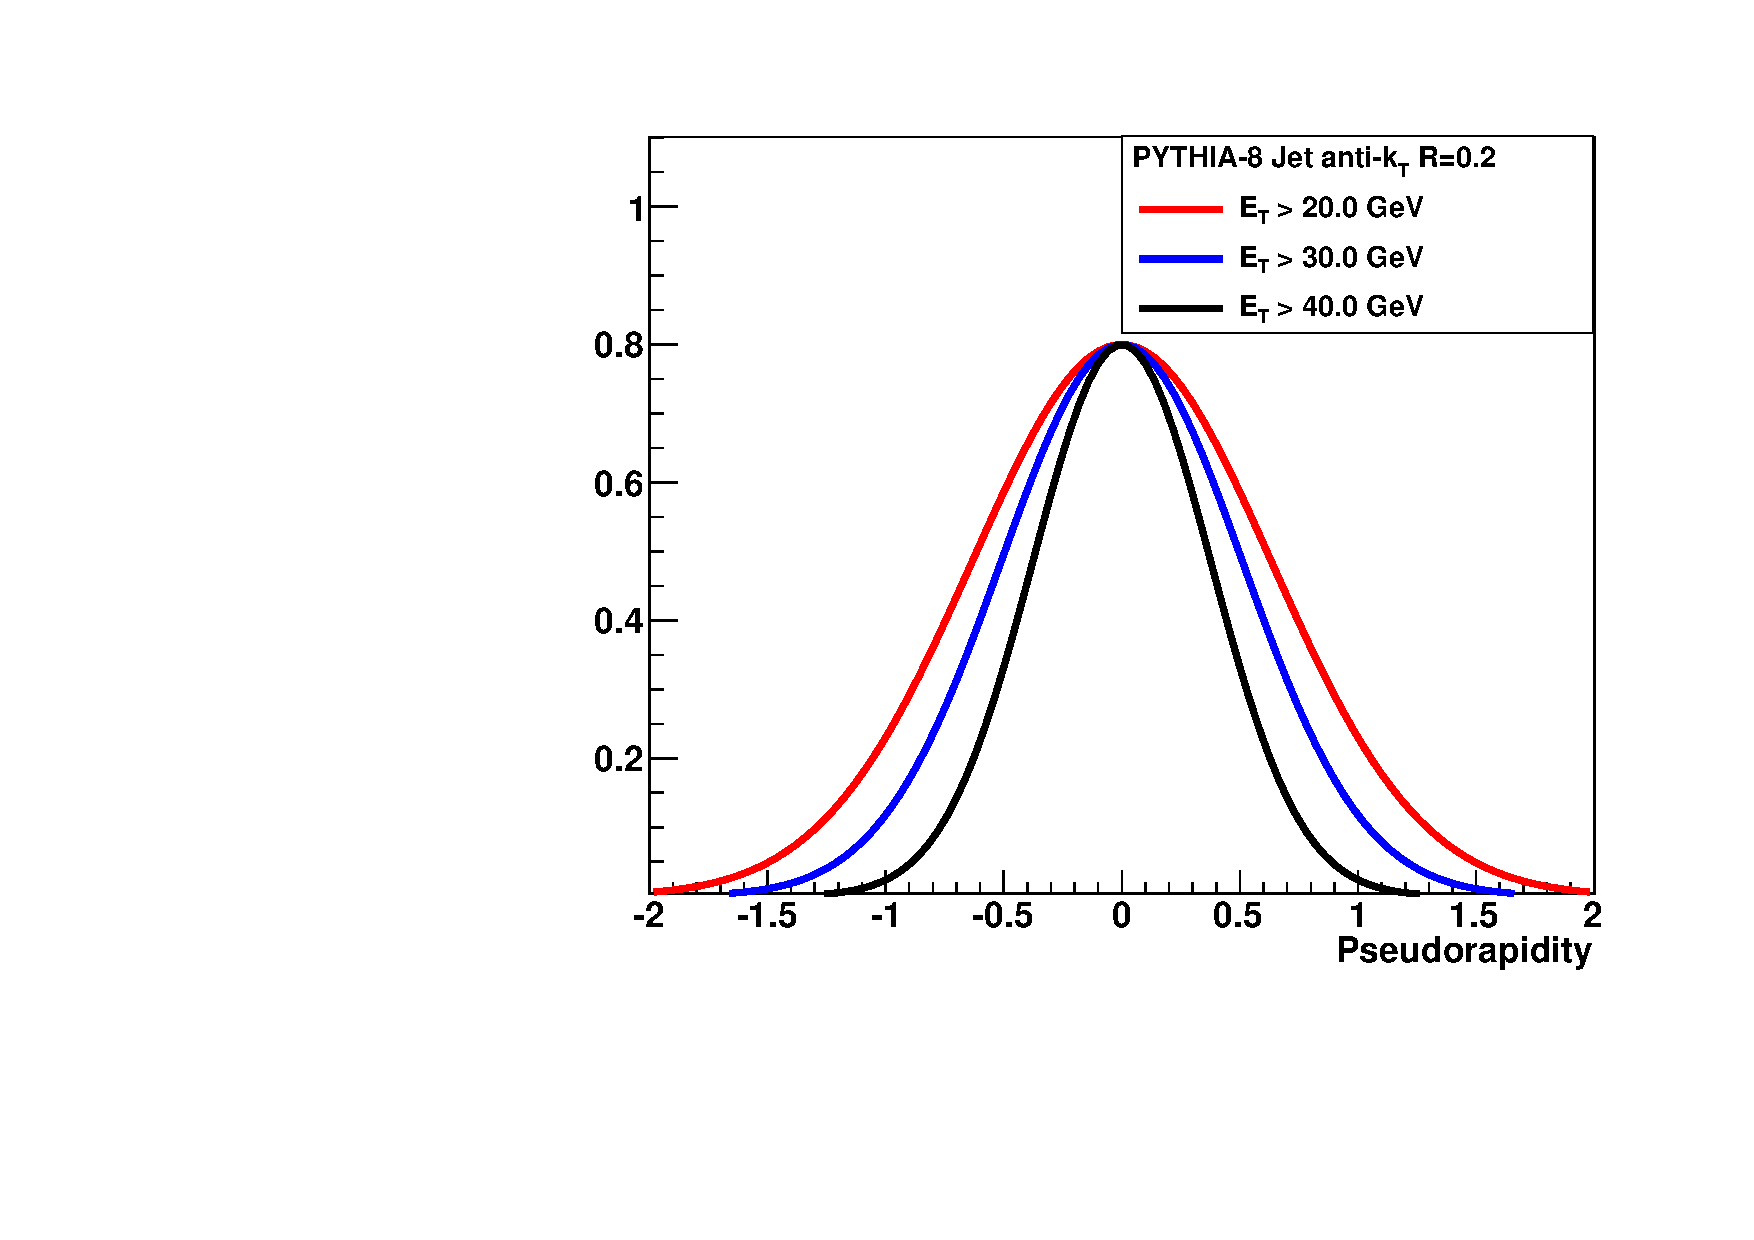
\includegraphics[trim = 2 2 2 2, clip, width=0.53\linewidth]{figs/figure_detectorrequirements_jetetadist}}
  \hfill
  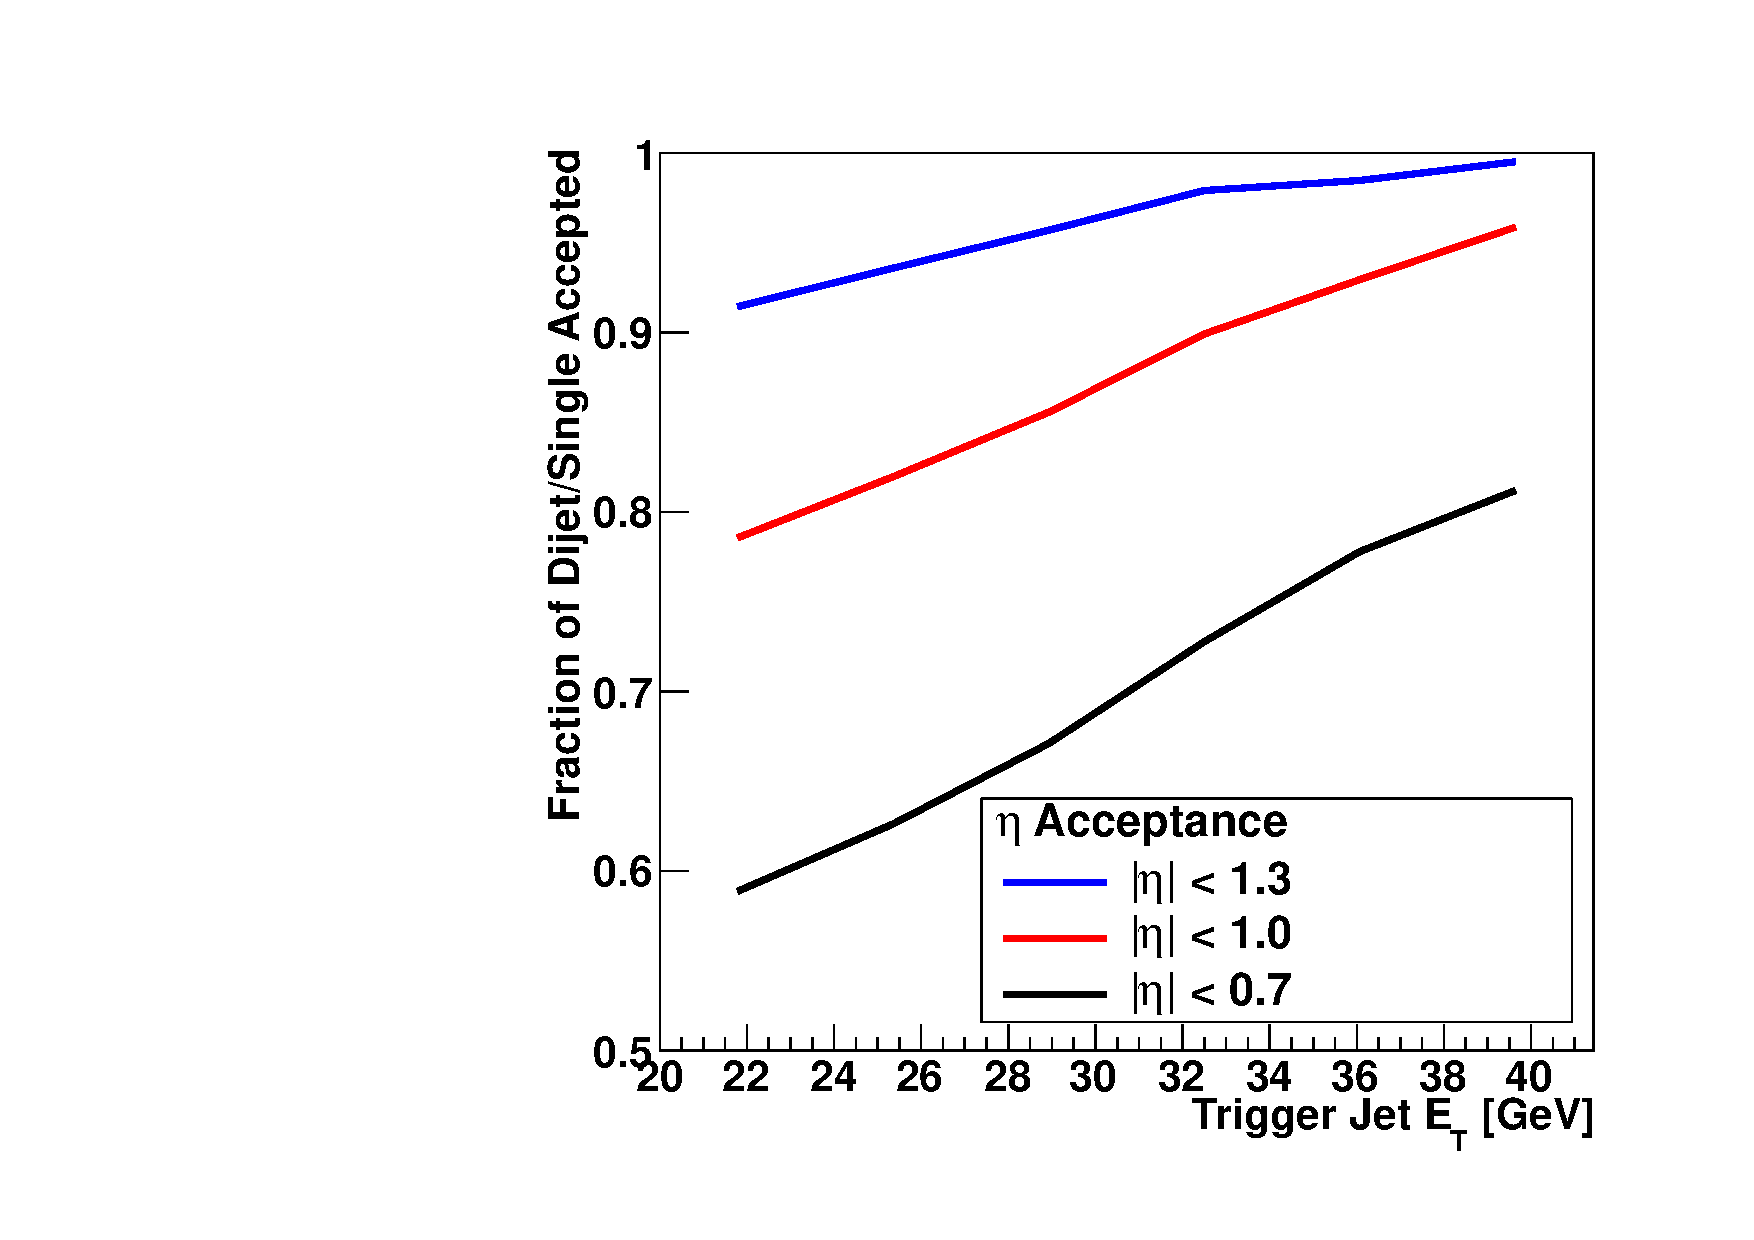
\includegraphics[trim = 2 2 2 2, clip, width=0.45\linewidth]{figs/figure_detectorrequirements_dijetaccept}
  \caption[Pseudorapidity distribution of \pythia jets reconstructed
  with the \fastjet anti-k$_{T}$ and the fraction of events in which
  the leading and subleading jet are in the specified
  acceptance]{\label{fig:pythia_dijet_accept}(Left) Pseudorapidity
    distribution of \pythia jets reconstructed with the \fastjet
    anti-k$_{T}$ and R=0.2 for different transverse energy selections.
    (Right) The fraction of \pythia events where the leading jet is
    accepted into a given pseudorapidity range where the opposite side
    jet is also within the acceptance. }
 \end{center}
\end{figure}

\subsection{Second subsection}


%\section {(Template) Section 2}
%\label{section2}
%The ECCE detector is a cylindrical detector covering
$\left|\eta\right| \leq 1.1$ and the full azimuth.  It is designed to use
the former BaBar superconducting solenoid to contain
an inner tracking system out to 80~cm in radius followed by an
electromagnetic calorimeter and the first of two longitudinal segments of
a hadronic calorimeter, which is not instrumented in the project baseline.  The second
longitudinal segment of the hadronic calorimeter, which is instrumented to
$|\eta| \leq 1.1$, also serves as
the magnet flux return, surrounding the magnet cryostat.

\subsection{Acceptance}

The large acceptance and high rate of ECCE are key enablers of the ECCE 
physics program~\cite{Adcox:2001jp}.
%%detailed in Chapter~\ref{sci_obj_perf}.  
The total
acceptance of the detector is determined by the requirement of high
statistics jet measurements and the need to fully contain both single
jets and dijets.  To fully contain hadronic showers in the detector
requires both large solid angle coverage and a calorimeter deep enough
to fully absorb the energy of hadrons up to 70~GeV.


\subsection{Second subsection}


\listoftodos[To Do]

\bibliographystyle{unsrturl}
\bibliography{refs}

\end{document}  %%%%%%%%%%%%%%%%% End Document
